\documentclass[a4paper,14pt]{report}
\usepackage[english,russian]{babel}
\usepackage{setspace}
\usepackage[unicode]{hyperref}
\usepackage[utf8]{inputenc}
\usepackage{xcolor}
\usepackage{amsmath}
\usepackage{wasysym}
\usepackage{latexsym}
\usepackage{indentfirst}
\usepackage{mathtools}
\definecolor{linkcolor}{rgb}{0.0,0.0,0.0}
\definecolor{urlcolor}{rgb}{0.0, 0.0, 0.0}
% \hypersetup{pdfstartview=FitH, linkcolor=linkcolor,urlcolor=urlcolor, colorlinks=true}
\usepackage[14pt]{extsizes}
\usepackage[
    left=30mm,
    top=20mm,
    right=10mm,
    bottom=20mm
]{geometry}
\usepackage{graphicx}
\usepackage{amsfonts}       % blackboard math symbols
\usepackage{subfigure}
\usepackage{afterpage}
\usepackage{titlesec}
\usepackage{float}
\usepackage{listings}
\usepackage{csquotes}
\usepackage{mathrsfs}
\usepackage{amssymb}
\usepackage{caption}
% \linespread{1.8}
% figure caption type changed
\captionsetup{labelsep=space}
\addto\captionsrussian{\renewcommand{\figurename}{Рисунок}}
% chapter settings
\titleformat{\chapter}[display]   
{\centering\Large\bfseries}{\chaptertitlename\ \thechapter}{10pt}{\Large}   
\titlespacing*{\chapter}{5pt}{-20pt}{30pt}


% section settings
\titleformat{\section}[block]
  {\large\bfseries}
  {\thesection\ }{0pt}{}

% settings for chapters and sections
\addto\captionsrussian{% Replace "english" with the language you use
  \renewcommand{\contentsname}%
    {\centering \large ОГЛАВЛЕНИЕ}%
  \renewcommand{\chaptername}{ГЛАВА}
  \renewcommand{\chaptertitlename}{ГЛАВА}
  \renewcommand{\bibname}{\large СПИСОК ИСПОЛЬЗОВАННОЙ ЛИТЕРАТУРЫ}
}

\renewcommand{\baselinestretch}{1.2}

\begin{document}
\setcounter{page}{1}
\setstretch{1.0}
\thispagestyle{empty}
\newgeometry{
    left=30mm,
    top=20mm,
    right=10mm,
bottom=20mm
}
\begin{center}
    \makebox[\textwidth][s]{\textbf{МИНИСТЕРСТВО ОБРАЗОВАНИЯ РЕСПУБЛИКИ БЕЛАРУСЬ}}
\end{center}
\begin{center}
    \textbf{БЕЛОРУССКИЙ ГОСУДАРСТВЕННЫЙ УНИВЕРСИТЕТ}
\end{center}
\begin{center}
    \textbf{Факультет прикладной математики и информатики}
\end{center}
\begin{center}
    Кафедра компьютерных технологий и систем
\end{center}

\vspace{3em}

\begin{center}
    ЛАРИН\\
    \vspace{-0.2cm}
    Егор Сергеевич
\end{center}
% \vspace{1cm}
\textbf{\begin{center}
        АНАЛИЗ И РАЗРАБОТКА РАСПРЕДЕЛЁННОЙ АРХИТЕКТУРЫ ЭКСПЛУАТАЦИИ НЕЙРОННЫХ СЕТЕЙ
    \end{center}}

\begin{center}
    Дипломная работа
\end{center}

\vfill

\begin{flushright}
    \begin{tabular}{@{}l@{}}
        Научный руководитель:             \\
        старший преподаватель кафедры     \\
        компьютерных технологий и систем \\
        Шолтанюк Станислав Витальевич
    \end{tabular}
\end{flushright}

\begin{flushleft}
    Допущен к защите\\
    «\underline{\hspace{1cm}}» \underline{\hspace{3cm}} 2024 г.\\
    \vspace{0.25cm}
    Зав. кафедрой компьютерных технологий и систем\\
    кандидат физ.-мат. наук, доктор педагогических наук\\
    профессор В. В. Казаченок
\end{flushleft}

\begin{center}
    Mинск, 2024
\end{center}

\clearpage
\restoregeometry
% \begin{center}
  \large\bfseries{РЕФЕРАТ}
\end{center}

Дипломная работа, 54 стр., 10 источников.

\textbf{Ключевые слова:} микросервисы, приложения с нейронными сетями, разработка программного обеспечения.

\textbf{Объекты исследования --} методы разработки масштабируемых приложений для эксплуатации нейронных сетей.

\textbf{Цель исследования --} систематизировать подходы к разработке микросервисов, выделить и применить ключевые методы разработки для приложений с нейронными сетями.

\textbf{Методы исследования --} изучение соответствующей литературы и электронных источников, постановка задачи и её решение.

\textbf{В результате исследования --} раскрыты и графически проиллюстрированы основные понятия микросервисной разработки, разработано приложение для генерации изображений.

\textbf{Области применения --} компьютерные технологии.

\newpage

\begin{center}
  \large\bfseries{ABSTRACT}
\end{center}

Thesis, 54 pages, 10 sources.

\textbf{Keywords:} microservices, neural network applications, software development.

\textbf{Objects of research --} methods for developing scalable applications for the implementation of neural networks.

\textbf{Aim of the study --} to systematize approaches to the development of microservices, identify and apply key development methods for neural network applications.

\textbf{Methods of research --} study of relevant literature and electronic sources, problem setting and its solution.

\textbf{Results of the study --} revealed and graphically illustrated the main concepts of microservice development, developed an application for image generation.

\textbf{Fields of application --} computer technologies.

\newpage

\begin{center}
  \large\bfseries{РЭФЕРАТ}
\end{center}

Дыпломная праца, 54 старонкі, 10 крыніц.

\textbf{Ключавыя словы:} мікрасервісы, прылады з нейроннымі сеткамі, распрацоўка праграмнага забеспячэння.

\textbf{Аб'екты даследвання --} метады распрацоўкі маштабуемых прылад для эксплуатацыі нейронных сетак.

\textbf{Мэта даследвання --} сістэматызацыя падыходаў да распрацоўкі мікрасервісаў, вылучэнне і прымяненне асноўных метадаў распрацоўкі для прылад з нейроннымі сеткамі.

\textbf{Метады даследвання --} вывучэнне адпаведнай літаратуры і электронных крыніц, пастаноўка задачы і яе рашэнне.

\textbf{Вынікі даследвання --} раскрыты і графічна ілюстраваны асноўныя паняцці мікрасервіснай распрацоўкі, распрацавана прылада для генерацыі малюнкаў.

\textbf{Сферы выкарыстання --} камп'ютэрныя тэхналогіі.

\newpage
\tableofcontents
\chapter*{\large ВВЕДЕНИЕ}  
\addcontentsline{toc}{chapter}{ВВЕДЕНИЕ}
В последние годы микросервисная архитектура значительно приобретает популярность в области разработки программного обеспечения.
Основная идея микросервисов заключается в разбиении сложных программных систем на отдельные,
слабо связанные компоненты с целью обеспечения гибкости, упрощения процессов разработки и масштабирования.
однако, эффективное управление такими многочисленными и взаимодействующими сервисами предполагает 
наличие централизованного описания и систематизированного подхода к их разработке и поддержке.

Наравне с развитием инструментов разработки программного обеспечения для веб-приложений 
широкое распространение получили также технологии, связанные с глубоким обучением. Нейронные сети могут решать широкий спектр
задач, но требуют значительного количества вычислительных ресурсов, что ставит перед разработчиками задачу построения
отказоустойчивых и масштабируемых систем, которые обрабатывают запросы для нейронных сетей.

Целью данной работы является описание существующих подходов к разработке микросервисных архитектур приложений, разработка 
масштабируемой и надежной архитектуры для инференса изображений с помощью нейронных сетей, описание трудностей, которые
возникают в процессе разработки и обозначение возможных путей решения подобных проблем.

В процессе исследования рассмотрены существующие методы, инструменты и подходы,
применяемые для проектирования микросервисных архитектур, приведены архитектуры нейронных сетей, которые используются для генерации
изображений, и разработана система, удовлетворяющая критериям микросервисной
архитектуры для генерации изображений из пользовательских запросов.


\chapter{Генерация изображений с помощью методов машинного обучения}
\section{Диффузионные нейронные сети для генерации изображений}

Генерация изображений с помощью нейронных сетей сегодня играет важную роль в развитии
информационных технологий, позволяя автоматизировать создание иллюстраций.
Широкое распространение генеративных технологий стало возможно благодаря улучшению методов обучения нейронных
сетей, которые решают данную задачу, и развитию вычислительной техники.

Выделяют различные виды задач генерации изображений:
\begin{enumerate}
  \item Генерация изображений по заданному текстовому описанию (промпту), которую в англоязычной литературе называют inpainting.
  \item Генерация фона по промпту, которую в англоязычной литературе называют outpainting. Обе перечисленных
  задачи сокращенно называют text2image.
  \item Генерация изображений по заданному изображению и промпту, которая находит применение в фильтрах обработки фотографий с помощью нейронный сетей. 
\end{enumerate}

При использовании текстовых промптов в качестве входных данных в первую очередь решается задача представления текста в виде векторов
чисел. 
Для этого используются токенайзеры, возможно, в комбинации с небольшими языковыми моделями.
Данный этап также представляет ценность на этапе обучения и позволяет распознавать запросы на разных языках и системах
письменности без использования нормализации и перевода.

В данной работе в первую очередь рассматривалась задача inpainting на примере маленьких открытых моделей семейства
stable diffusion, поскольку они позволяют продемонстрировать основные проблемы, связанные с инференсом изображений
при высокой нагрузке, но не требуют больших вычислительных ресурсов и просты в эксплуатации.

Одним из значимых методов обучения нейронных сетей, предназначенных для генерации изображений, стал Generative adversarial network (GAN).
Ключевой особенностью данного метода на этапе обучения является наличие двух глубоких нейронных сетей: $G(z)$, которая по распределению $p_g$ ставит
в соответствие векторам $z$ изображения $x$, и сети $D(x)$, которая возвращает скалярное значение,
которое является вероятностью того, что $x$ является реальным изображением, то есть является частью
обучающей выборки. 
Основная идея процесса обучения заключается в минимизации величины $\log (1 - D(G(z)))$, что означает, что $G$ пытается «обмануть» дискриминатор $D$.
Поэтому подобный подход к обучению нейронный сетей можно считать обучением без учителя. 

Таким образом процесс получения распределения $p_g$ можно представить в виде игры с нулевой суммой двух игроков
с критерием \cite{gan}
$$
\min_{G}\max_{D} V(D, G) = \mathbf{E}_{x~p_{data}(x)}[\log D(x)] + \mathbf{E}_{z~p_{z}(z)}[\log (1 - D(G(z)))]
$$ 

Данный подход гарантирует сходимость при увеличении обучающей выборки и обеспечивает хорошую скорость инференса относительно подходов,
основанных на других вероятностных методах, но является очень трудозатратным при обучении модели.

Поэтому наряду с GAN часто применяются диффузионные модели (Diffusion models), принцип которых основан на 
итеративном извлечении шума с изображения, что позволяет создавать из шума искомые изображения.
\section{Латентные диффузионные нейронные сети для генерации изображений}


Важную роль процессе уменьшения шума в изображении играет сегментация изображений с помощью U-Net нейронных сетей,
которые имеют большое значение в биоинформатике.

Основная идея U-Net заключается в последовательном использовании блоков конволюции и деконволюции вместе с ReLU 
функциями активации (Рисунок \ref{fig:unet}), при котором разрешение исходного изображения последовательно понижается, а потом повышается
до исходного. 


\begin{figure}[H]
  \centering
  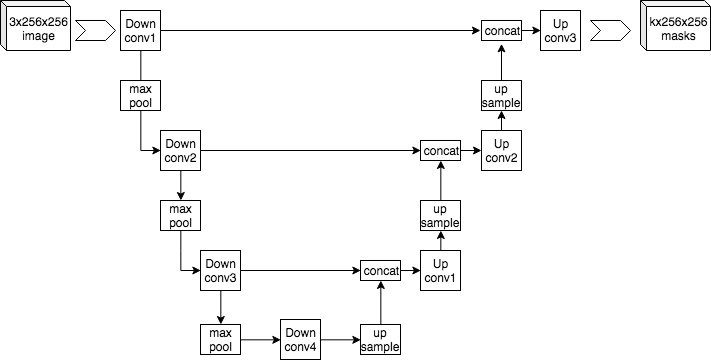
\includegraphics[width=0.95\textwidth]{img/unet.png}
  \caption{U-Net \cite{rombach2022high}}
    \label{fig:unet}
\end{figure}


В результате данных преобразований на изображении выделяются основные детали, соответствующие отдельным объектам (Рисунок \ref{fig:conv}), а полученное изображение,
как правило, называют маской. В контексте использования диффузионных моделей для генерации изображений использование
сегментации на зашумленных изображений помогает более эффективно избавляться от шума, что улучшает сходимость процесса генерации.

\begin{figure}[H]
  \centering
  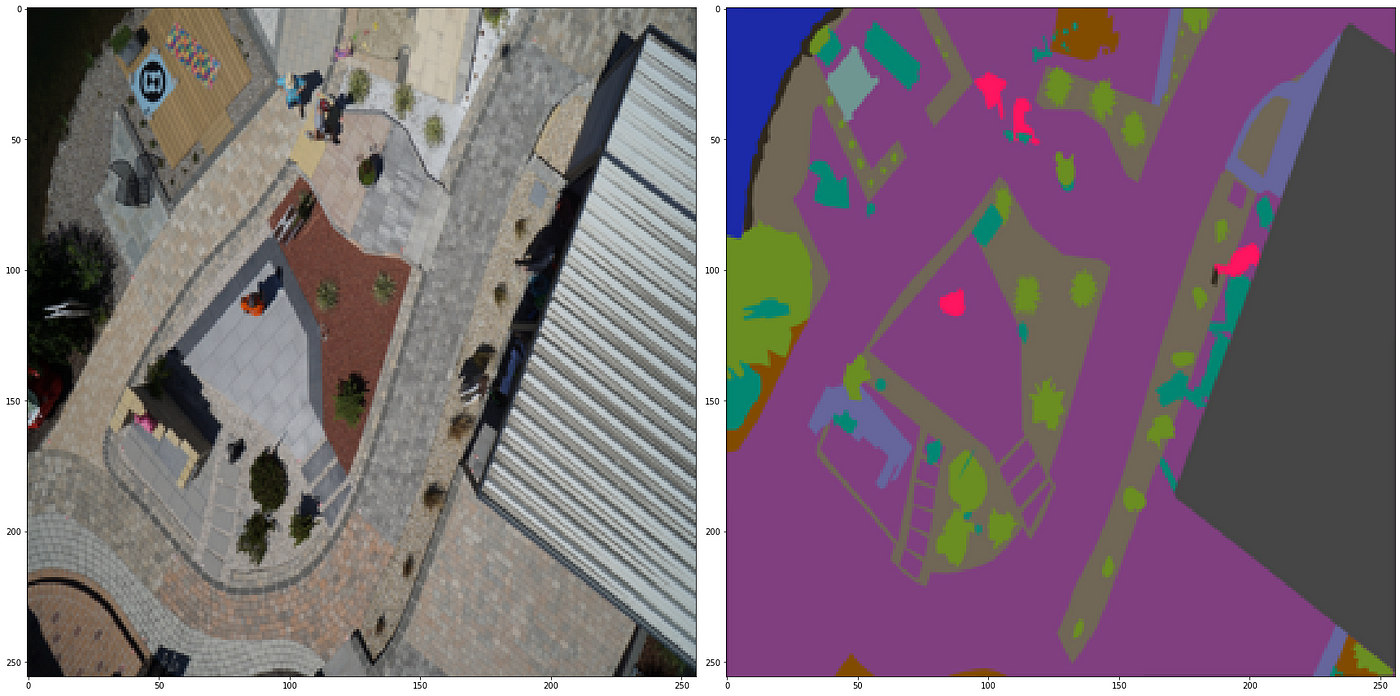
\includegraphics[width=0.95\textwidth]{img/conv.png}
  \caption{Результат примения U-Net на изображении}
    \label{fig:conv}
\end{figure}

Комбинацию подходов сегментации изображений между шагами генерации зачастую выделяют в отдельный тип нейронных сетей, называемый
латентными диффузионными моделями (Latent Diffusion Models). Латентными их называют за счет того, что латентным называют пространство
изображений, получаемых в ходе шагов семплирования, с применением конволюции и деконволюции U-Net. Это значительно
упрощает обучение модели и позволяет сразу генерировать изображения в высоком разрешении против подходов, где применяется
комбинация нескольких нейронных сетей, где на определенных шагах формируются детали, а на конечных повышается разрешение
до искомого (Рисунок \ref{fig:latent}).
LDM лежат в основе большинства современных нейронных сетей,
которые решают задачу генерации изображений, таких как DALLE, Midjourney и YandexART.
\begin{figure}[H]
  \centering
  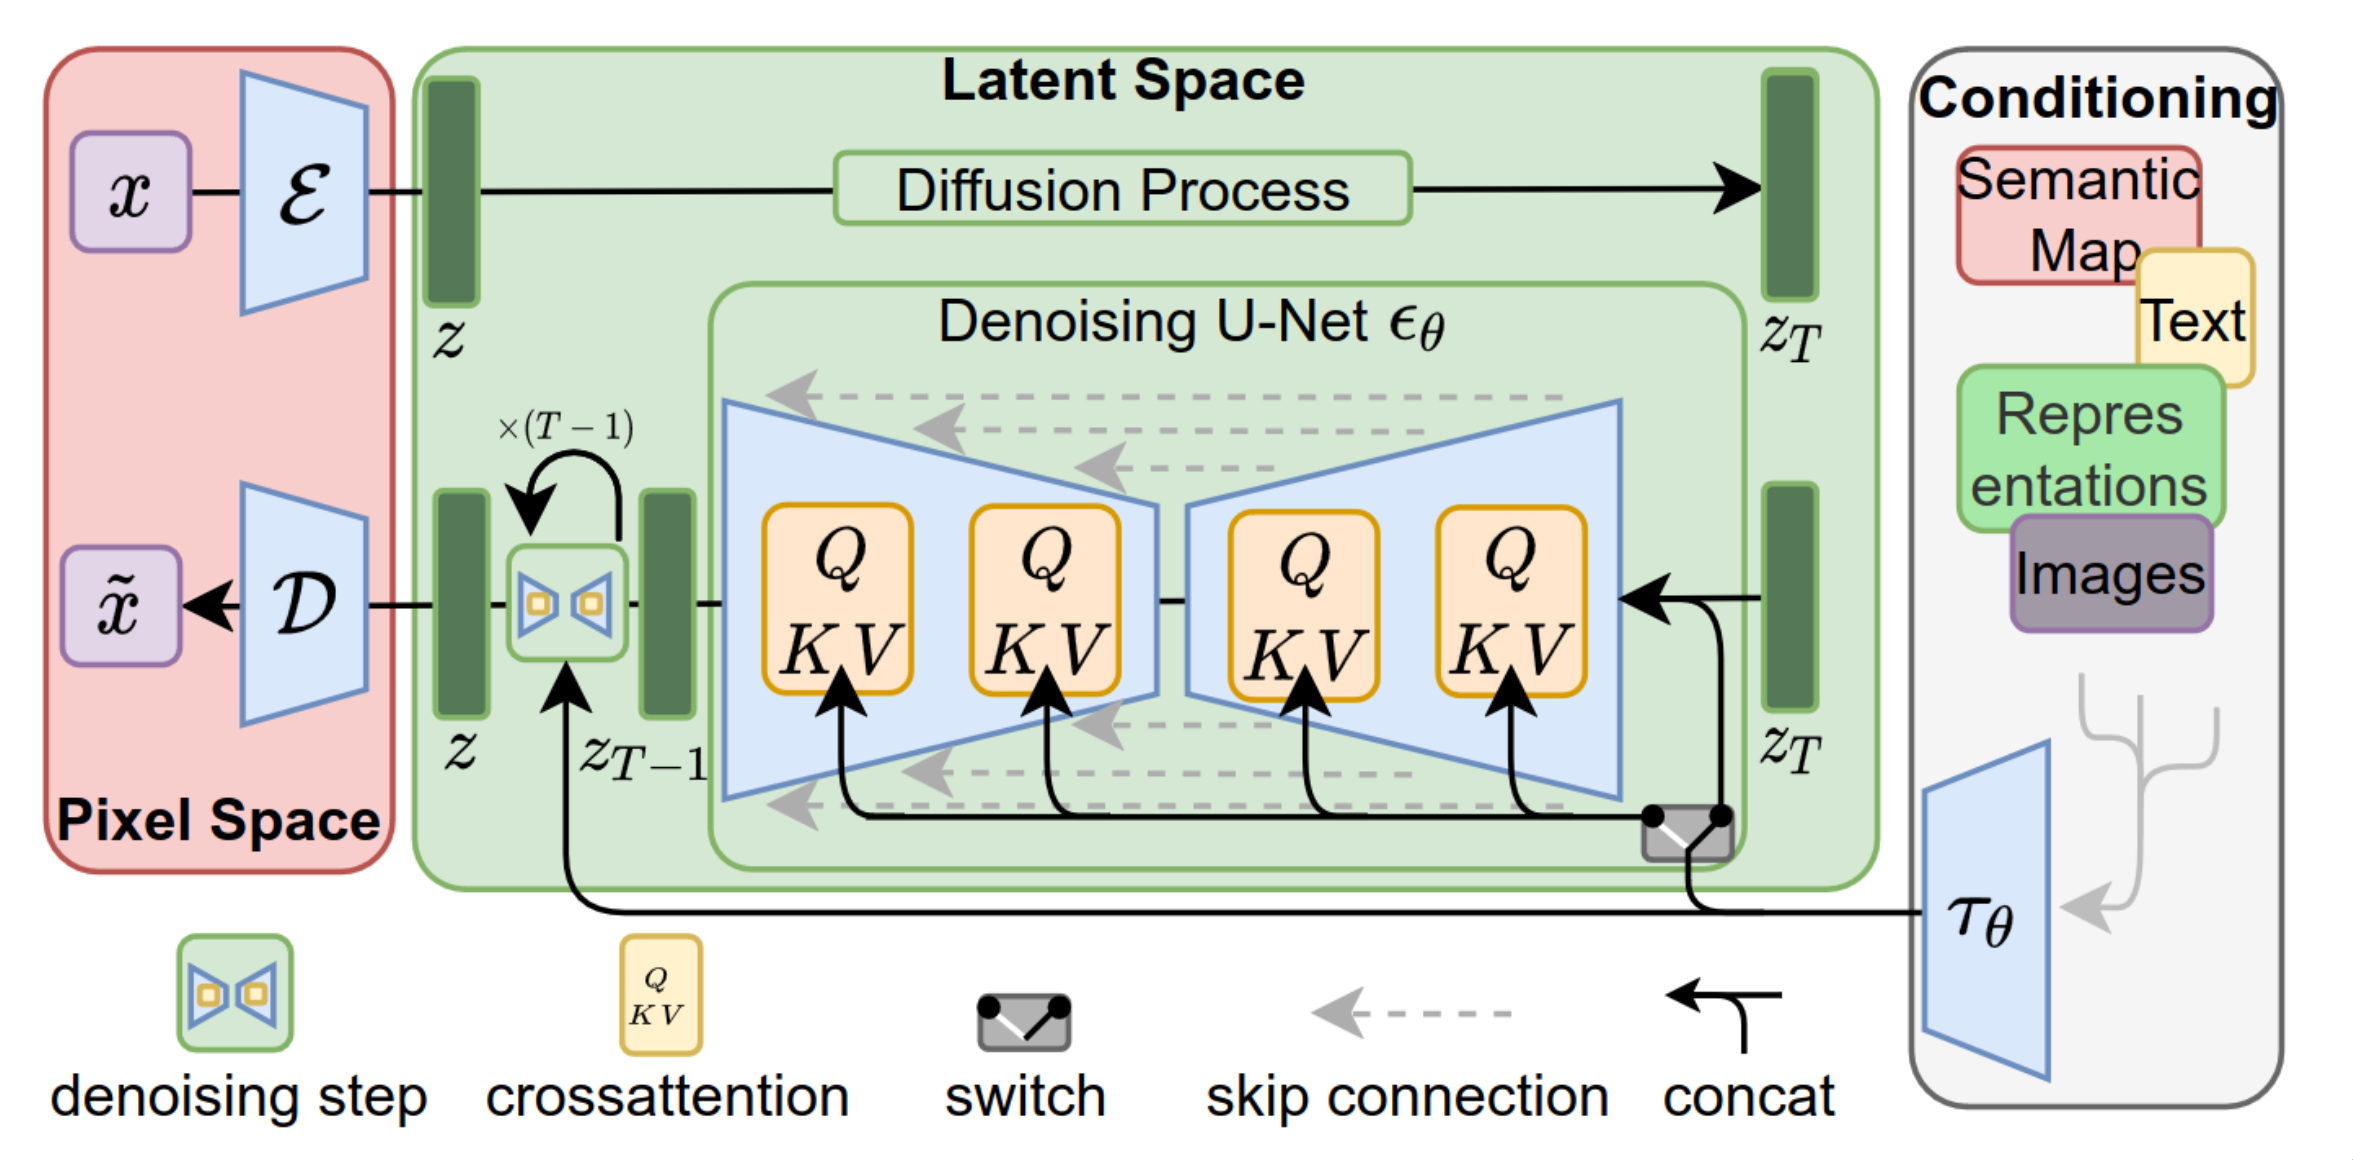
\includegraphics[width=0.95\textwidth]{img/latent.png}
  \caption{Схема архитектуры LDM\cite{rombach2022high}}
    \label{fig:latent}
\end{figure}

Несмотря на применение вышеперечисленных оптимизаций,
генерация высококачественных изображений доступна только на высокопроизводительных GPU промышленнного сегмента,
представленными, например, NVidia V100, A100, H100 и так далее. 
Данные вычислительные устройства производятся в ограниченном количестве и являются относительно дорогими,
что делает невозможным обработку множества запросов в режиме реального времени, что требует выстроения инфраструктуры
вокруг моделей, которая сможет обеспечить бесперебойную и асинхронную обработку сообщений, 
соответствующую по пропускной способности количеству вычислительных ресурсов.
Также при большом количестве RPS (requests per second) на генерацию встает вопрос о масштабирования кластера
видеокарт. 

Одним из возможных сценариев масштабирования вычислительных ресурсов является создание суперкомпьютеров с объединением
шины данных нескольких видеокарт. Подобные технологии представлены в потребительском сегменте технологиями SLI от компании NVidia и CrossFire от AMD, однако
данные технологии в первую очередь предназначены для неспециализированных вычислений, которые, например, нужны для
отрисовки графики в видеоиграх и не всегда подходят для сложных вычислительных задач, а так же не предоставляют достаточную скорость
обмена данными между видеокартами. Подобные подходы так же критикаются за счет того, что производительность таких систем не растет линейно и
требуют высоких накладных расходов на синхронизацию работы нескольких видеокарт.

Поэтому в качестве альтернативного способа создания кластеров видеокарт зачастую применют технологию NVLink, разработанную 
компанией NVidia (Рисунок \ref{fig:nvlink}). Она не предназначена для решения задач общего назначения, поэтому видеокарты с поддержкой NVlink не всегда обладают 
мультимедийными интерфейсами, типа HDMI или DisplayPort, однако предоставляет в 3 раза большую частоту передачи данных
по сравнению с видеокартами с интерфейсом подключения PCIExpress 3.0 на примере видеокарт серии V100.

Данный подход может обеспечить максимальную производительность за счет минимизации передачи данных по сети
и предоставляет самый эффективный механизм вертикального масштабирования. Объединение видеокарт в кластеры на аппаратном
уровне может быть необходимостью при обучении больших моделей или инференсе моделей, которые не помещаются целиком
в память одной видеокарты, однако может быть излишним для инференса небольших, до 40-80 гигабайт, обученных моделей,
поскольку проектирование подобной системы на физическом уровне может быть очень затратным и имеет пределы, диктуемые
сетевой аппаратурой и контролерами, в которые подключается кластер видеокарт.

\begin{figure}[H]
  \centering
  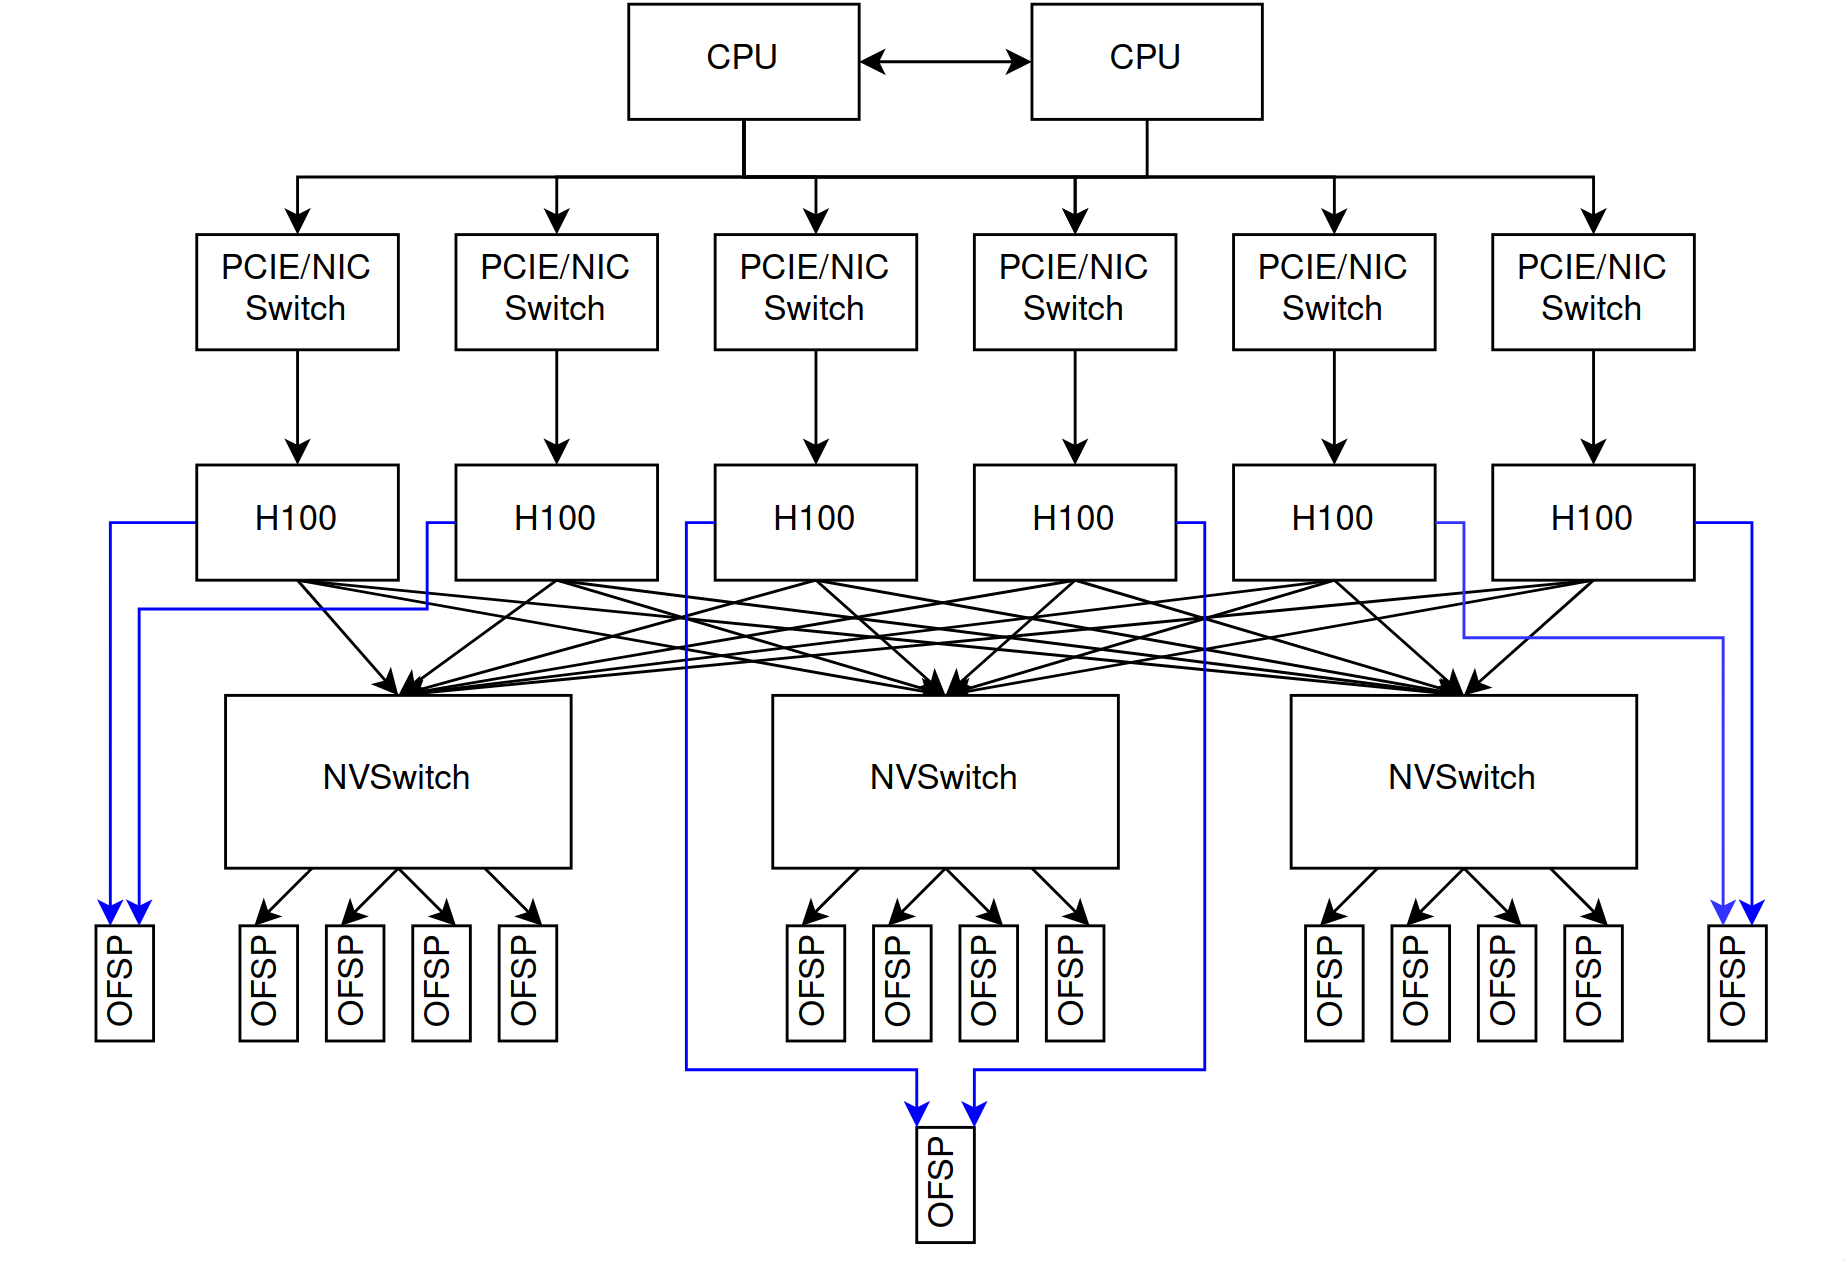
\includegraphics[width=0.95\textwidth]{img/nvlink.png}
  \caption{NVlink кластер}
    \label{fig:nvlink}
\end{figure}


В качестве альтернативы аппаратному кластеру видеокарт можно использовать архитектуру, в которой видеокарты не объединяются
в аппаратный кластер, а обладают независимыми шинами данных, а координация их работы обеспечивается на уровне приложения.
Данный подход позволяет разнести вычислительные ресурсы на разные машины и не требует более сложной инфраструктуры, связанной
с обслуживанием оборудования, соответсвенно, предоставляет более простые механизмы горизонтального масштабирования,
что может помочь в построении больших систем. Видеокарты, которые работают по отдельности, также не нуждаются в 
NVlink и могут быть подключены через более дешевый и простой в эксплуатации PCIExpress.
С другой стороны, такой подход может не подойти для сценариев, где модель не помещается в память одной видеокарты, и координация
работы составной нейронной сети будет медленнее, чем в системе с несколькими видеокартами, за счет необходимости
передачи данных по сети. Еще можно заметить, что видеокарты предназначенные для PCIExpress обладают более медленной
памятью, поэтому, на примере видеокарт H100, при одинаковых характеристиках чип будут показывать худшую производительность
при решении вычислительных задач.

В случае если к системе не предъявляется вышеперечисленных требований, предпочтительным является именно этот подход за счет своей простоты.
Самым простым в реализации будет построение архитектуры, где общение с моделями осуществляется через балансер, который
держит ограниченный пул соединений с HTTP-серверами моделей. Обеспечение HTTP API для модели обеспечивается пользователем
на уровне приложения или используется готовое решение, типа TorchServe, который обеспечивает батчинг запросов и конфигурацию без
без необходимости реализации этого программистом.

\begin{figure}[H]
  \centering
  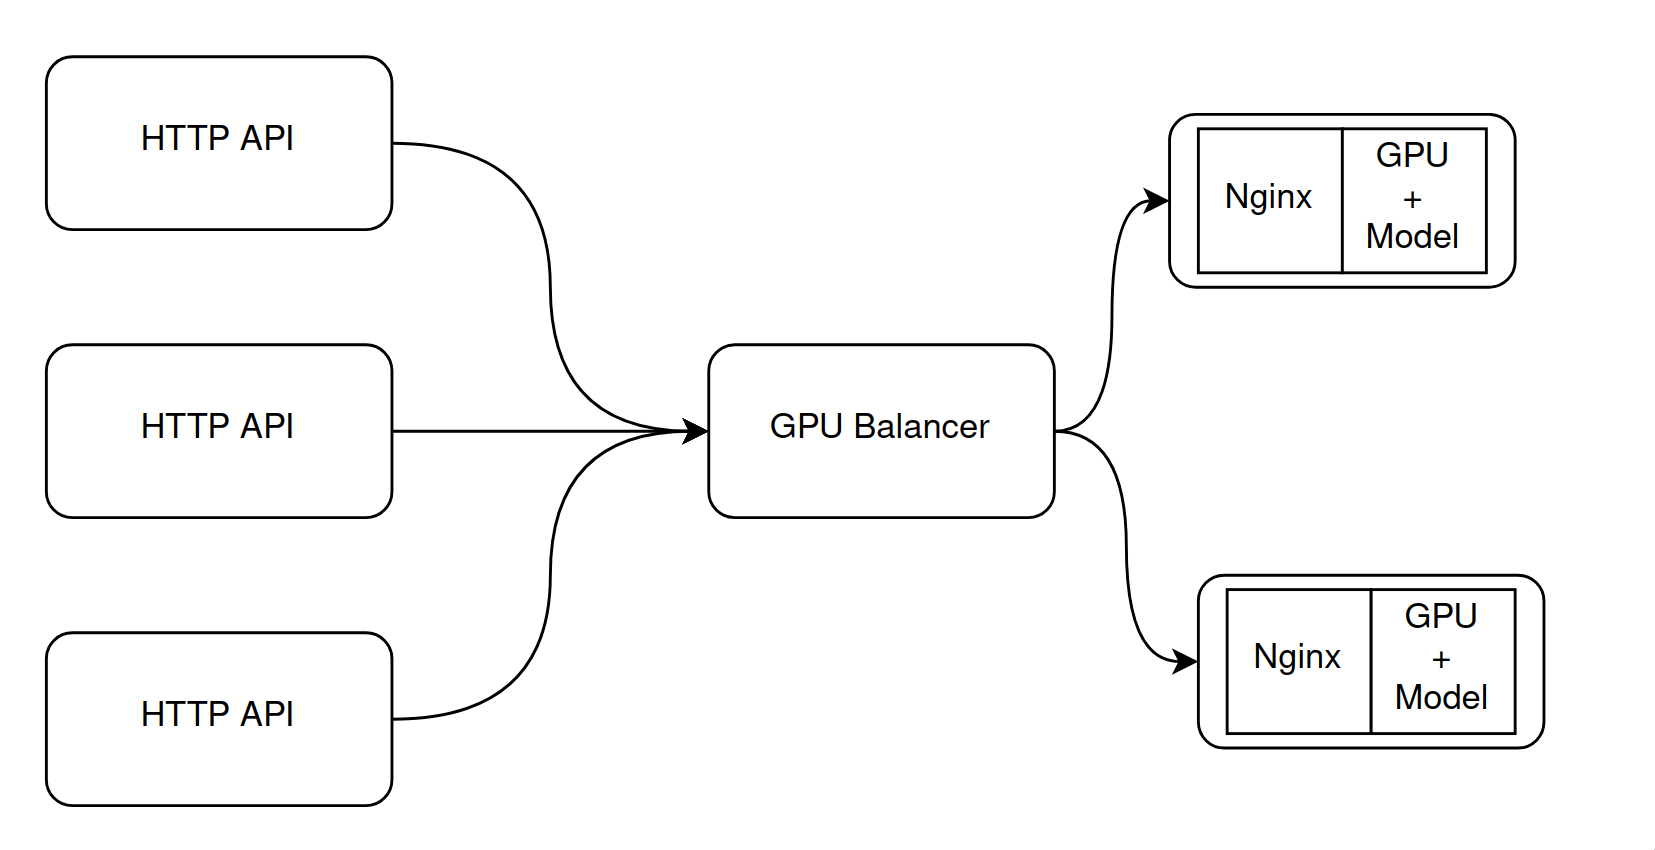
\includegraphics[width=0.95\textwidth]{img/gpu_balancer.png}
  \caption{Балансер}
    \label{fig:balancer}
\end{figure}

Использование общего балансера может упростить инфраструктуру системы и код для эксплуатации модели, однако налагает
серьезные ограничения на отказоустойчивость системы: при большом количестве RPS на генерацию может не хватать 
соединений, за счет того, что на каждый запрос, который не может быть обработан сразу из-за отсутствия свободных ресурсов,
будет выделено отдельное соединение, тратящее процессорное время. Также релизный цикл обновлений модели
будет требовать сложной конфигурации систем деплоя, типа Kubernetes, для обеспечения бесперебойной обработки запросов (Green-Blue Deployment).
Иначе текущие запросы будут обрываться в процессе обновлений.

В качестве альтернативы можно дополнить данную схему отдельной очередью, что позволит обрабатывать сообщения асинхронно, а 
гарантии обработки обеспечивать за счет механизмом подтверждения на уровне брокера сообщений, который выступает в роли очереди.

В данном случае HTTP-прокси будет заменен на интерфейс взаимодействия с брокером сообщений, написанный на языке 
рантайма инференса, или на другом языке программирования. В последнем случае обработка сообщений и инференс модели
будут происходить в разных процессах на одной физической модели, а приложения для взаимодействия с брокером сообщений называется 
Sidecar.

\begin{figure}[H]
  \centering
  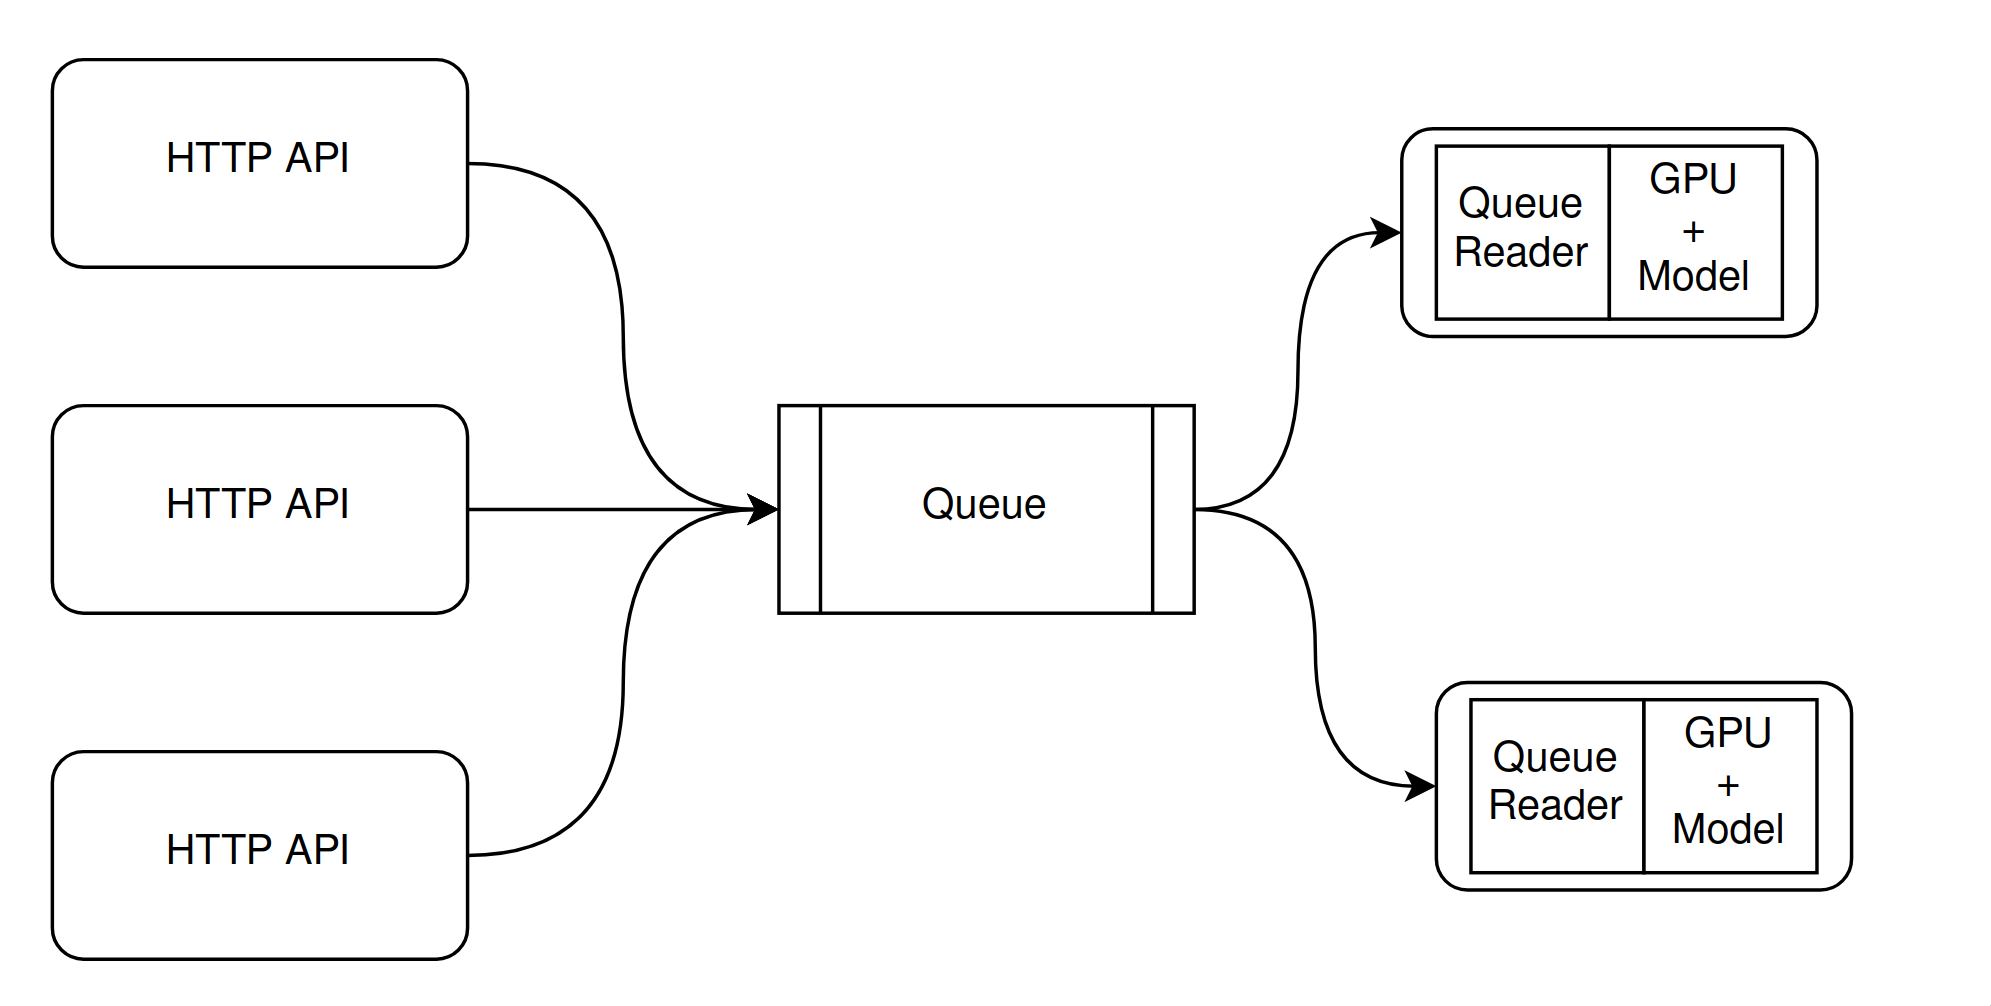
\includegraphics[width=0.95\textwidth]{img/queue.png}
  \caption{Очередь}
    \label{fig:queue}
\end{figure}

В качестве преимуществ данного подхода можно выделить более простую обработку сценариев с высокой нагрузкой
и обработкой ошибок на стороне модели за счет подтверждений на стороне брокера сообщений и его персистентного хранилища,
которое будет хранить информацию о запросе установленное время даже после перезапуска приложения. Использование
очереди также может обеспечить гарантии очередности обработки сообщений, что дает более предсказуемое время ожидания
под высокой нагрузкой. 

\chapter{ОБЗОР ОСНОВНЫХ ПОДХОДОВ ДЛЯ РЕАЛИЗАЦИИ МИКРОСЕРВИСОВ}
\section{Обзор микросервисной архитектуры}

Представление о микросервисах родилось в 2005 году из подхода SOA путем обобщения философии UNIX для веб-компонент.
Веб-сервисы сопоставляются независимым программам, комбинация которых осуществляется с помощью сетевого транспорта данных по аналогии с именованными и неименованными UNIX каналами.
В отличие от SOA микросервисы не фокусируются на конкретных форматах передачи данных, как SOAP, 
а дают представление о том, как должны коммуницировать сервисы, чтобы при сохранении слабой связности компонент поддерживать устоявшийся контракт обмена информацией \cite{micro-1}.

В современной литературе не существует одного конкретного определения микросервиса. 
Обычно микросервисы определяют через различные критерии соответствия распределенной системе с низкой связностью ее отдельных компонент.

Большое внимание в теории микросервисов уделяется вопросам масштабируемости. 
Для всестороннего описания масштабируемости в контексте разработки распределенных систем вводится понятие куба масшабируемости \cite{scalability} (Рисунок \ref{fig:cube}).

\begin{figure}[H]
    \centering
    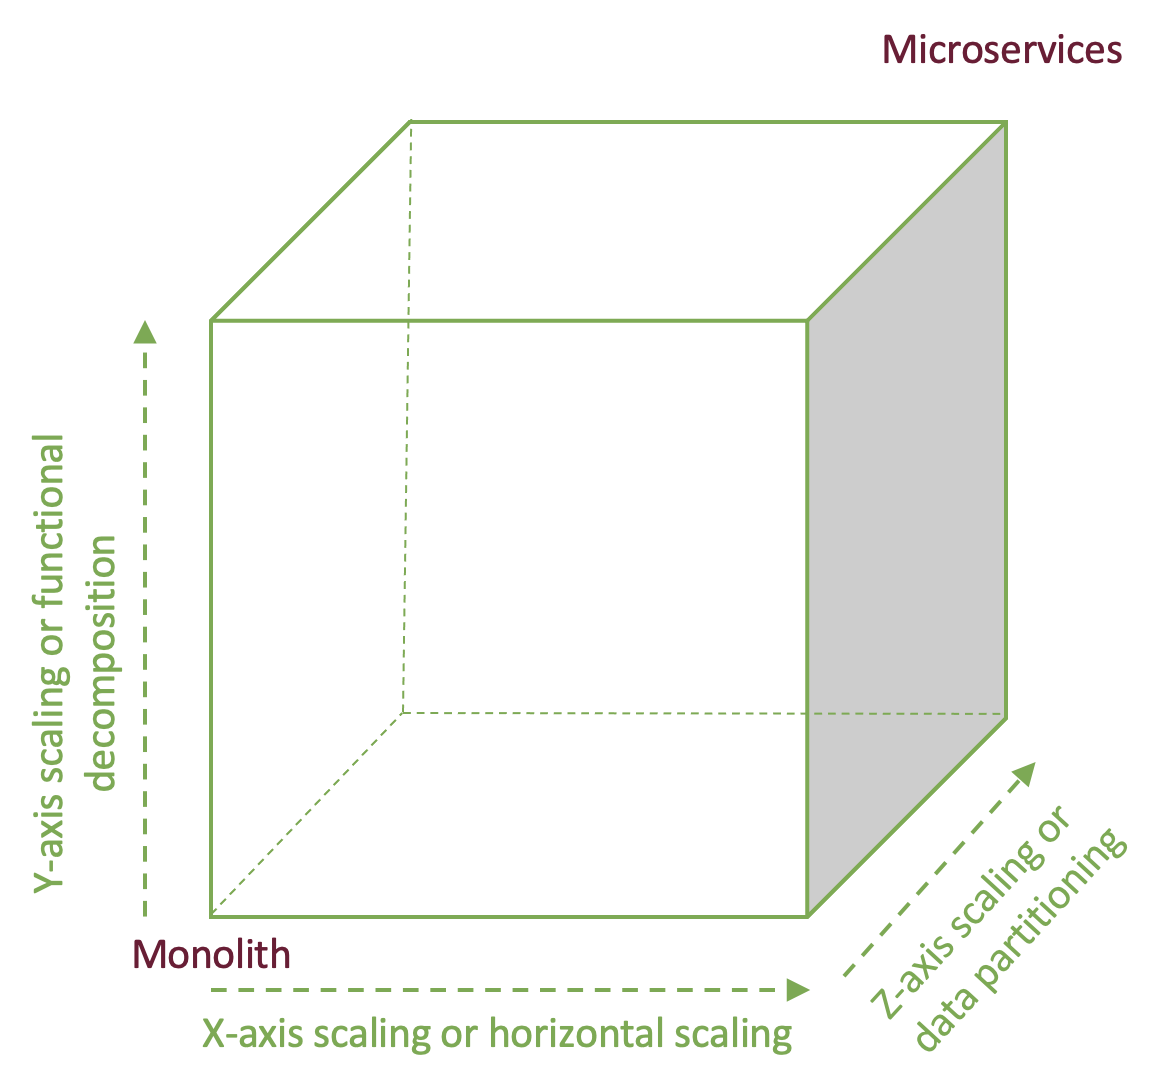
\includegraphics[width=0.4\linewidth]{img/cube.png}
    \caption{--- Куб масштабируемости}
    \label{fig:cube}
\end{figure}

Эта модель определяет три направления для масштабирования приложений: $X$, $Y$ и $Z$.

Масштабирование по оси X часто применяют в монолитных приложениях. 
Запускается несколько экземпляров программы, размещенных за балансировщиком нагрузки. 
Балансировщик распределяет запросы между $N$ одинаковыми экземплярами. 
Это распространенный способ улучшить
производительность и стабильность приложения.

Масштабирование по оси $Z$ тоже предусматривает запуск нескольких экземпляров
монолитного приложения, но в этом случае, в отличие от масштабирования по
оси $X$, каждый экземпляр отвечает за определенное подмножество данных.
Маршрутизатор, выставленный впереди, задействует атрибут запроса, чтобы на
править его к подходящему экземпляру. 

Масштабирование по осям $X$ и $Z$ увеличивает производительность и стабильность приложения.
Но ни один из этих подходов не решает проблем с усложнением кода и процесса раз
работки. Чтобы справиться с ними, следует применить масштабирование по оси $Y$,
или функциональную декомпозицию. То, как это работает, показано на рисунке \ref{fig:y}.
\begin{figure}[H]
    \centering
    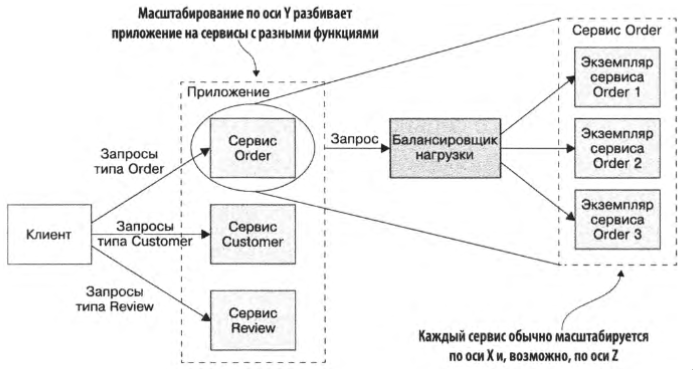
\includegraphics[width=0.8\linewidth]{img/y.png}
    \caption{--- Пример декомпозиции приложения через отдельные сервисы}
    \label{fig:y}
\end{figure}

Таким образом, сервис — это приложение, реализующее узкоспециализированные функции, такие как управление заказами, управление клиентами и т. д. 
Сервисы масштабируются по оси $X$, некоторые из них могут использовать также ось $Z$. Например,
сервис Order (Рисунок \ref{fig:y}) имеет несколько копий, нагрузка на которые балансируется.
Одно из обобщенных определение микросервисной архитектуры (или микросервисов)
звучит так: это стиль проектирования, который разбивает приложение на отдельные
сервисы с разными функциями. Заметим, что размер здесь вообще не упоминается.
Главное, чтобы каждый сервис имел четкий перечень связанных между собой обязанностей.

Микросервисная архитектура имеет следующие преимущества:
\begin{itemize}
    \item Она делает возможными непрерывные доставку и развертывание крупных, сложных приложений.
    \item Сервисы получаются небольшими и простыми в обслуживании.
    \item Сервисы развертываются независимо друг от друга.
    \item Сервисы масштабируются независимо друг от друга.
    \item Микросервисная архитектура обеспечивает автономность команд разработчиков.
    \item Она позволяет экспериментировать и внедрять новые технологии.
    \item В ней лучше изолированы неполадки других сервисов.
\end{itemize}

Одна из проблем, возникающих при использовании микросервисной архитектуры, связана с отсутствием конкретного, хорошо описанного алгоритма разбиения
системы на микросервисы. 
Что означает, что эта часть данной методологии, не имеет формального описания \cite{micro-1}. 

В связи с этим также выделяют понятие распределенного монолита.

Распределенным монолитом называют набор связанных между собой сервисов, которые необходимо развертывать вместе. Распределенному монолиту присущи недостатки
как монолитной, так и микросервисной архитектуры.

Еще один недостаток микросервисной архитектуры состоит в том, что при создании
распределенных систем возникают дополнительные сложности для разработчиков. 
Сервисы должны использовать механизм межпроцессного взаимодействия.

Это сложнее, чем вызывать обычные методы в общей памяти приложения. 
К тому же код должен уметь
справляться с частичными сбоями и быть готовым к недоступности или высокой
латентности удаленного сервиса.
Реализация сценариев, охватывающих несколько сервисов, требует применения
дополнительных технологий. 

\section{Практики использования СУБД в микросервисных архитектурах}

Для реализации надлежащего уровня изоляции между микросервисами применяется паттерн database per service.
В этом случае каждый микросервис имеет собственную базу данных при необходимости холодного хранилища данных. 
Это позволяет вносить правки в функциональность сервиса без риска сломать функциональность другого сервиса и привлечения других команд для согласования изменений, 
а также позволяет просто оценивать время ответов и нагрузку для каждого из сервисов по отдельности, что сложно осуществимо при использовании общих ресурсов.

Несмотря на вышеперечисленные преимущества упомянутого паттерна, database per service затрудняет реализацию комбинированных транзакций и запросов. 
Подобные операции по модификации данных в разных экземплярах баз данных называют распределенными транзакциями.
Возникновение распределенных транзакций в архитектуре приложения налагает ограничения на повторные запросы и хеджирование и усложняет
применение практик по повышению надежности системы, поскольку при повторных неиндемпотентных запросах или прерванных запросах на запись в несколько баз данных
может быть нарушена консистентность данных.
Для решения подобных проблем внедряются отдельные протоколы координации запросов в базы данных.

Примером подобного протокола является 2PC (two phase commit) -- двухфазный коммит. Этот протокол предполагает
наличие надежного координатора, который предоставляет общую точку синхронизации для разных сервисов, и откатывает изменения
во всех базах при возникновении ошибок в одном из узлов (Рисунок \ref{fig:twopc}).
\begin{figure}[H]
    \centering
    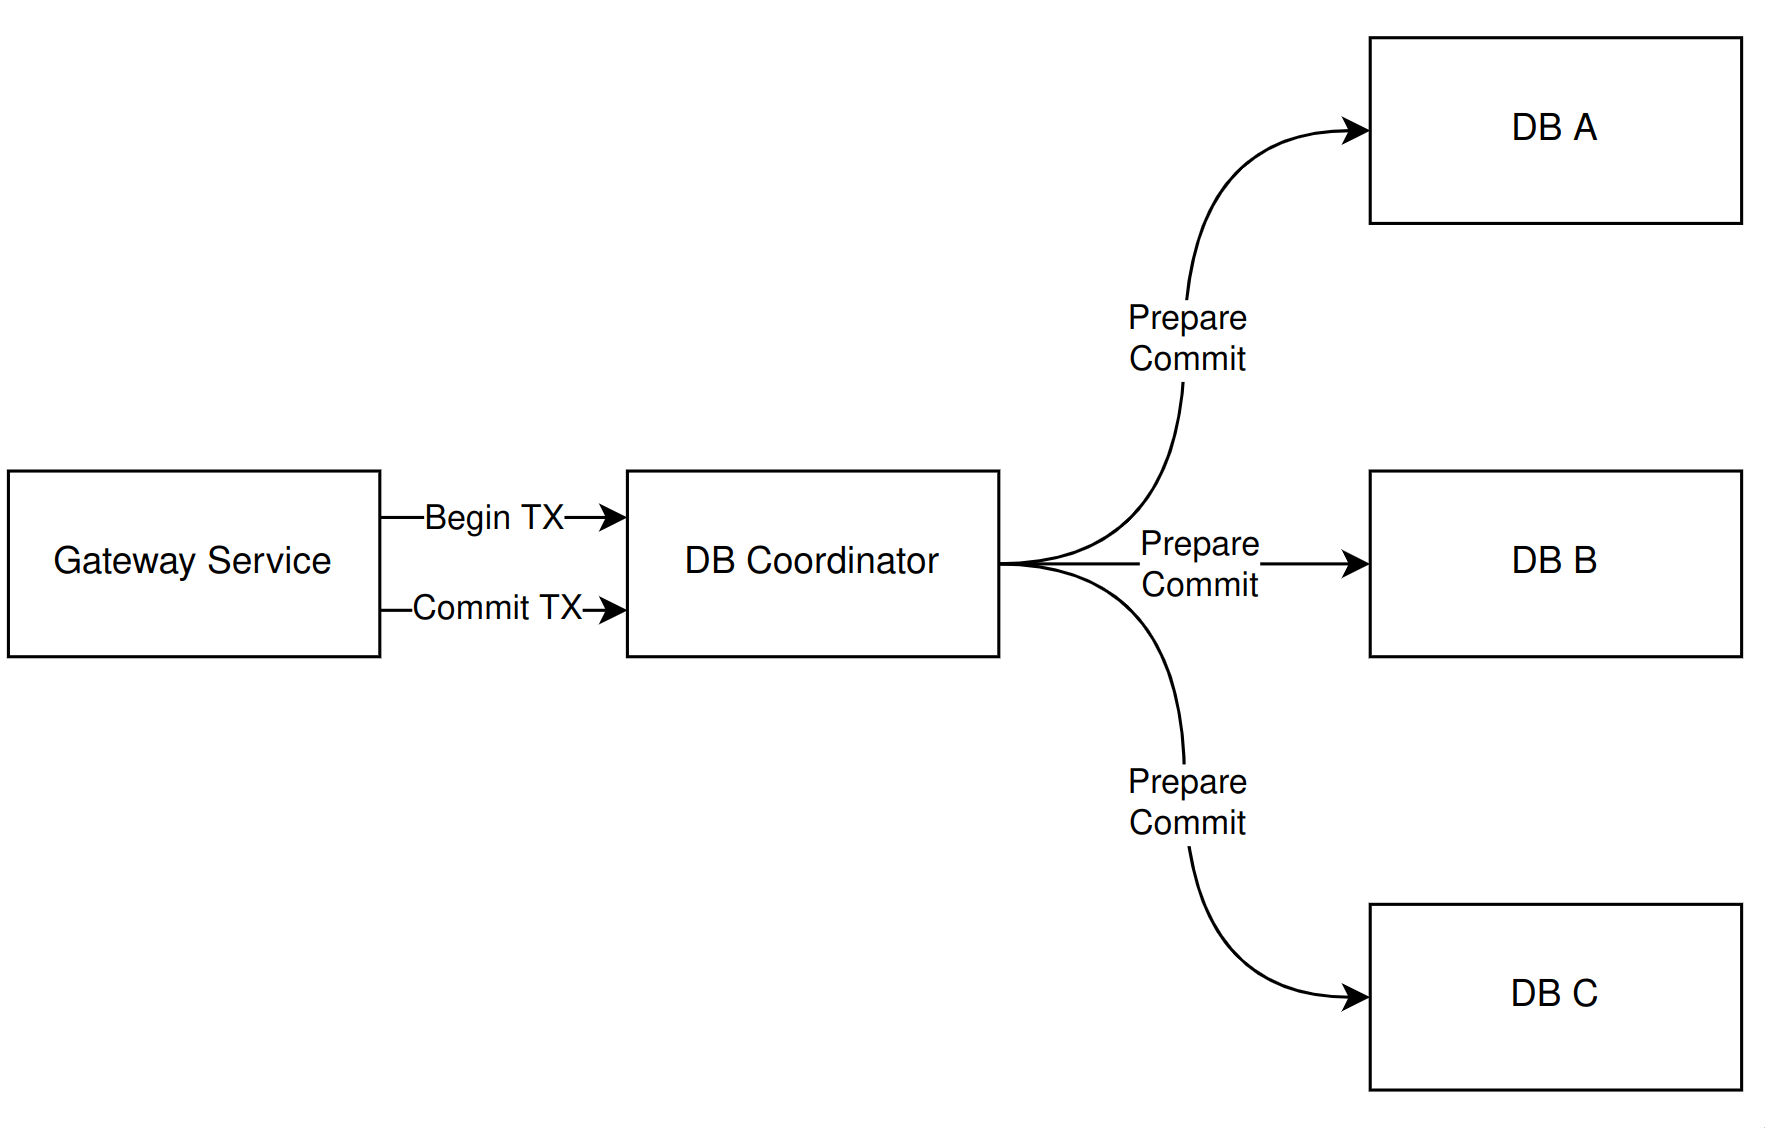
\includegraphics[width=0.8\linewidth]{img/2pc.png}
    \caption{--- Принцип работы 2PC}
    \label{fig:twopc}
\end{figure}

Несмотря на то, что протокол был разработан в 70-ые годы, он до сих используется в современных приложениях, например,
с помощью менеджера транзакций Narayana для платформы Spring. Многие базы данных также предоставляют достаточные механизмы транзакций, которые
требуются для реализации данного протокола. Подобные транзакции называют XA (Extend Architecture) транзакциями, которые обеспечивают
консистентность данных за счет дополнительной синхронизации.
В данном случае достигается максимально возможная консистентность данных, однако
необходимость в отдельном узле синхронизации снижает производительность, усложняет масштабирование из-за ограничений координатора, и конфигурация подобных систем
может быть довольно сложной.
Также данный протокол плохо применяется
для нереляционных баз данных, что неприемлемо для современных приложений.

Для решения вышеперечисленных проблем прибегают к паттерну Saga. В этом случае в качестве координатора
выступает один из сервисов (Рисунок \ref{fig:saga}), который осуществляет модификацию данных в других сервисах в рамках своих транзакций.
При возникновении ошибок на такой сервис-оркестратор возлагается ответственность вызвать нужные методы
для попытки сохранить или восстановить консистентность данных в других базах.

\begin{figure}[H]
    \centering
    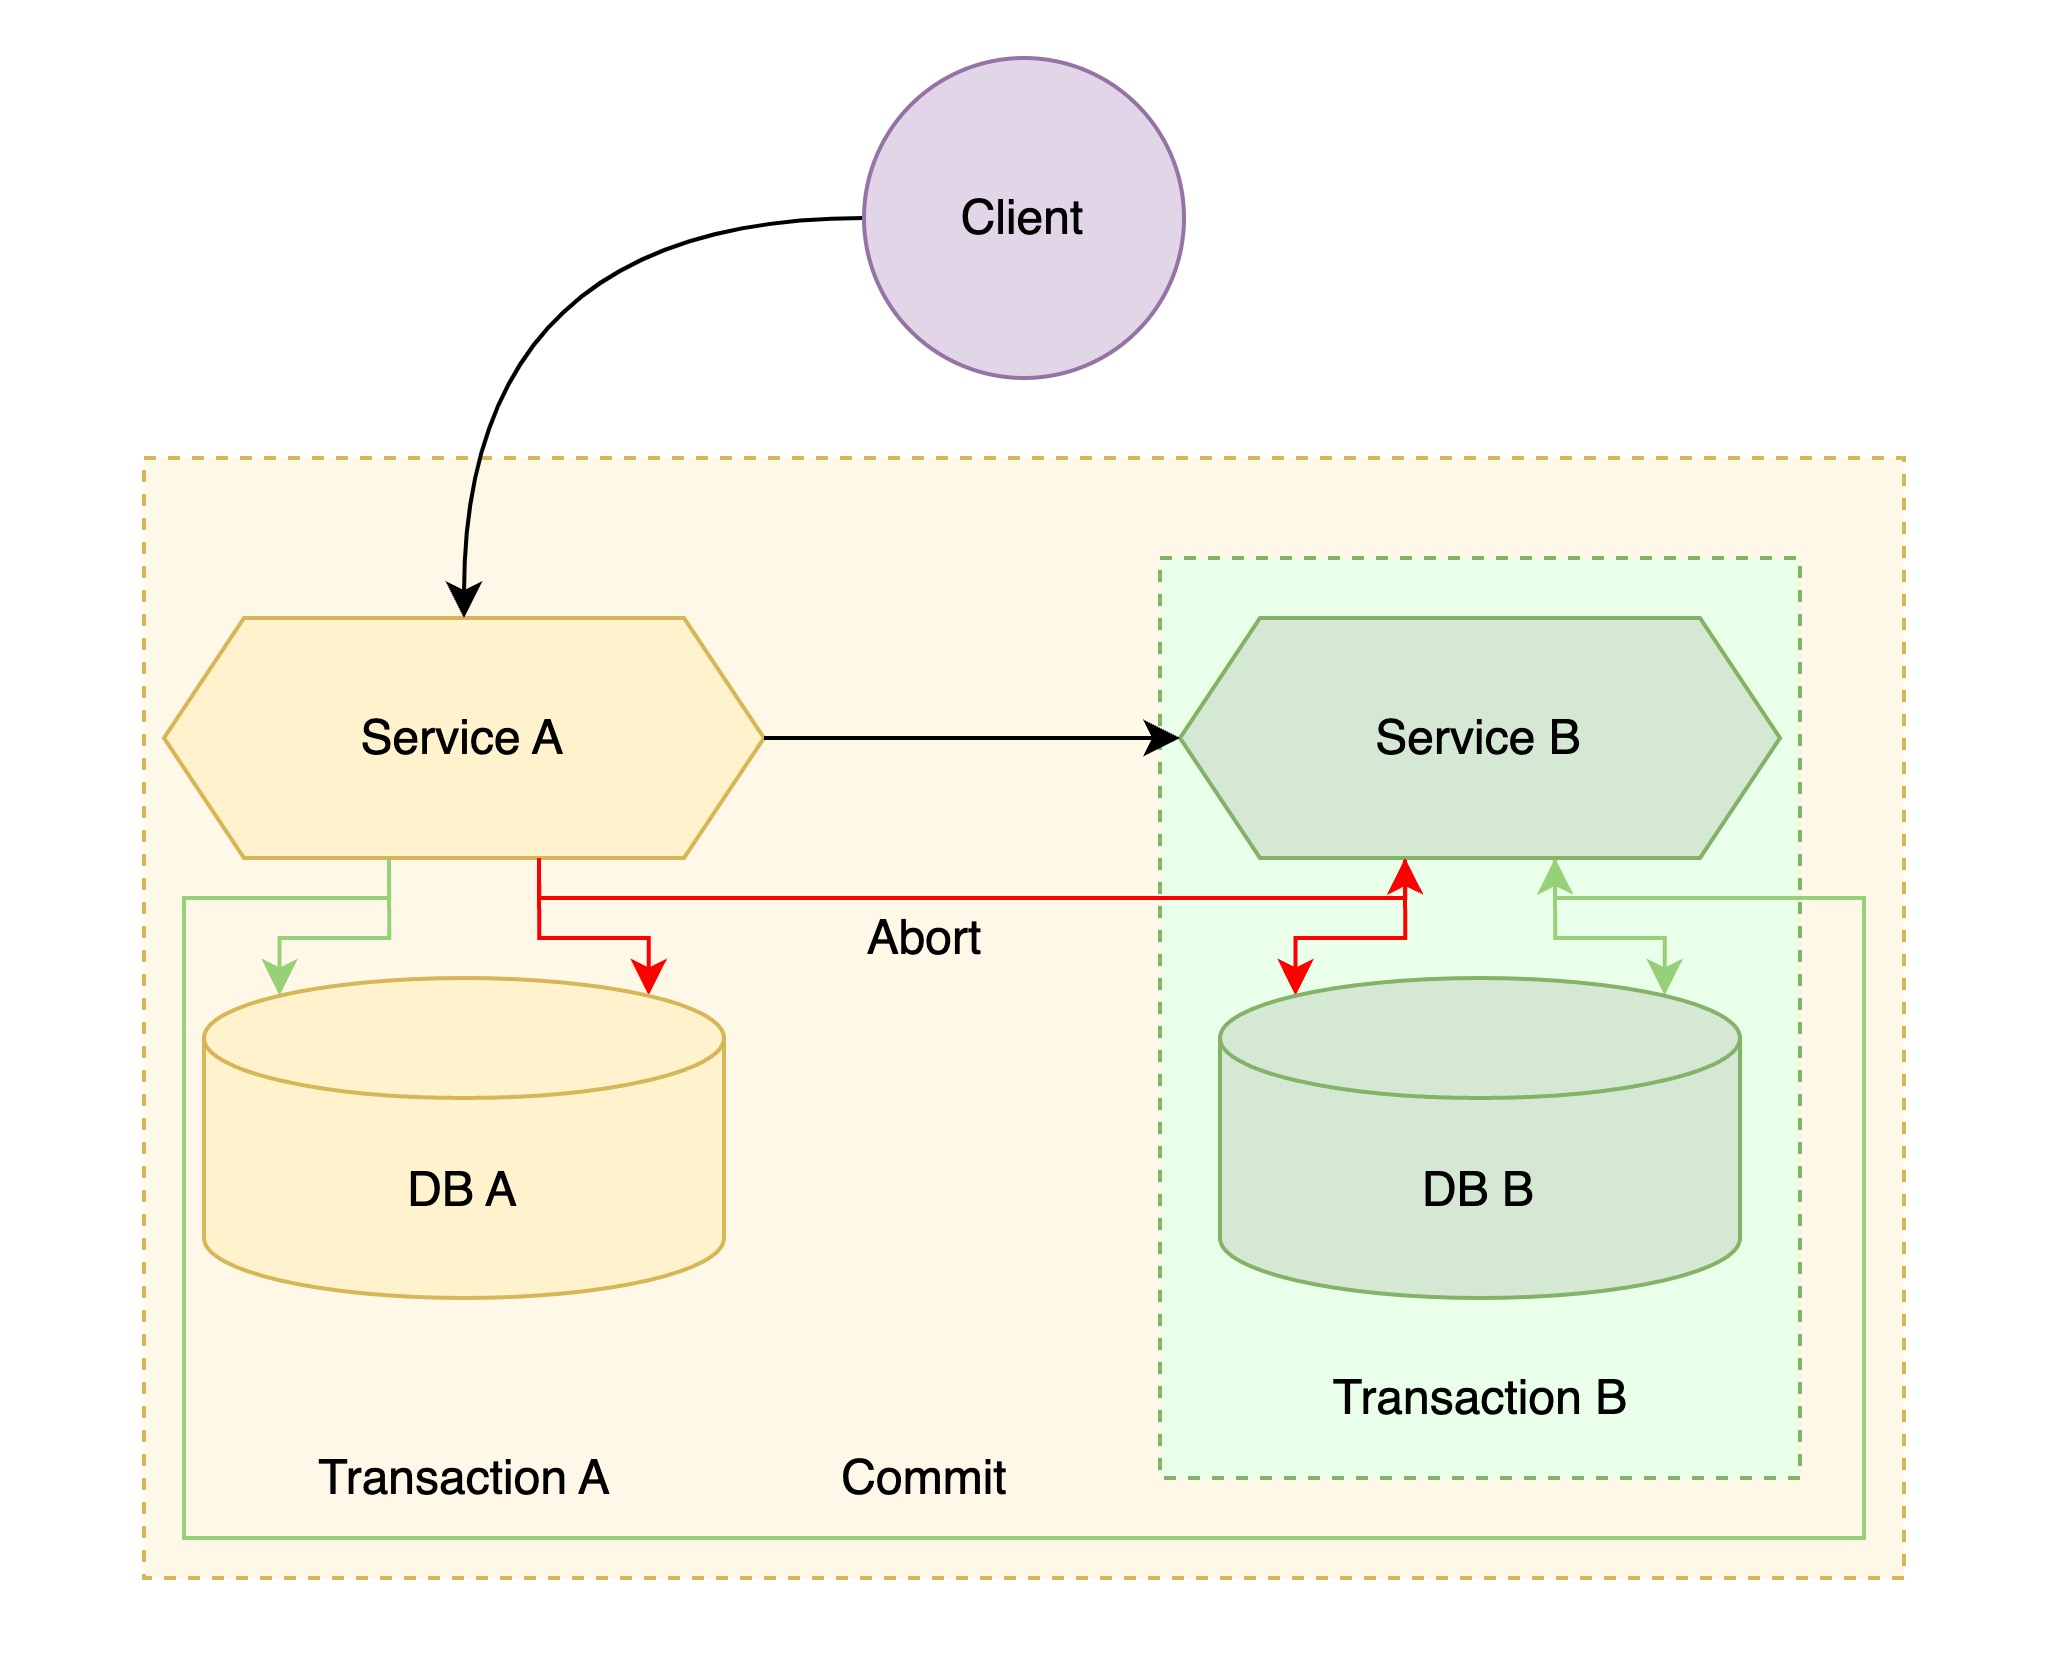
\includegraphics[width=0.8\linewidth]{img/saga.png}
    \caption{--- Принцип работы Saga}
    \label{fig:saga}
\end{figure}

При использовании одного из сервисов в качестве координатора уменьшаются задержки
коммуникации между сервисами и не требуются XA транзакции, что положительно сказывается на производительности
системы. Однако подобный подход не обеспечивает таких же гарантий консистентности данных, как 2PC или контроль над исполнением
транзакций в монолитном приложении. Поэтому может подойти для систем, где требования к производительности выше требований консистентности.

В качестве альтернативы также применют модификации Saga, где координатора может не быть вовсе. В этом
случае все операции модификации данных происходят асинхронно. Например, сервис, который раньше был координатором теперь может записывать
события, которые должны воспроизвести нужное состояние системы в отдельную очередь, которую читает другой сервис и самостоятельно управляет своими транзакциями.
В этом случае нет издержек на централизованное управление транзакций, а контроль над исполнением возлагается на механизмы обработки сообщений брокера (Рисунок \ref{fig:saga_async}).
Однако возникают проблемы с тем, что данные в базах данных больше не синхронизированы, 
и при отмене транзакции в одном сервисе после записи в очередь другой сервис может не получить об этом ответного сообщения.

\begin{figure}[H]
    \centering
    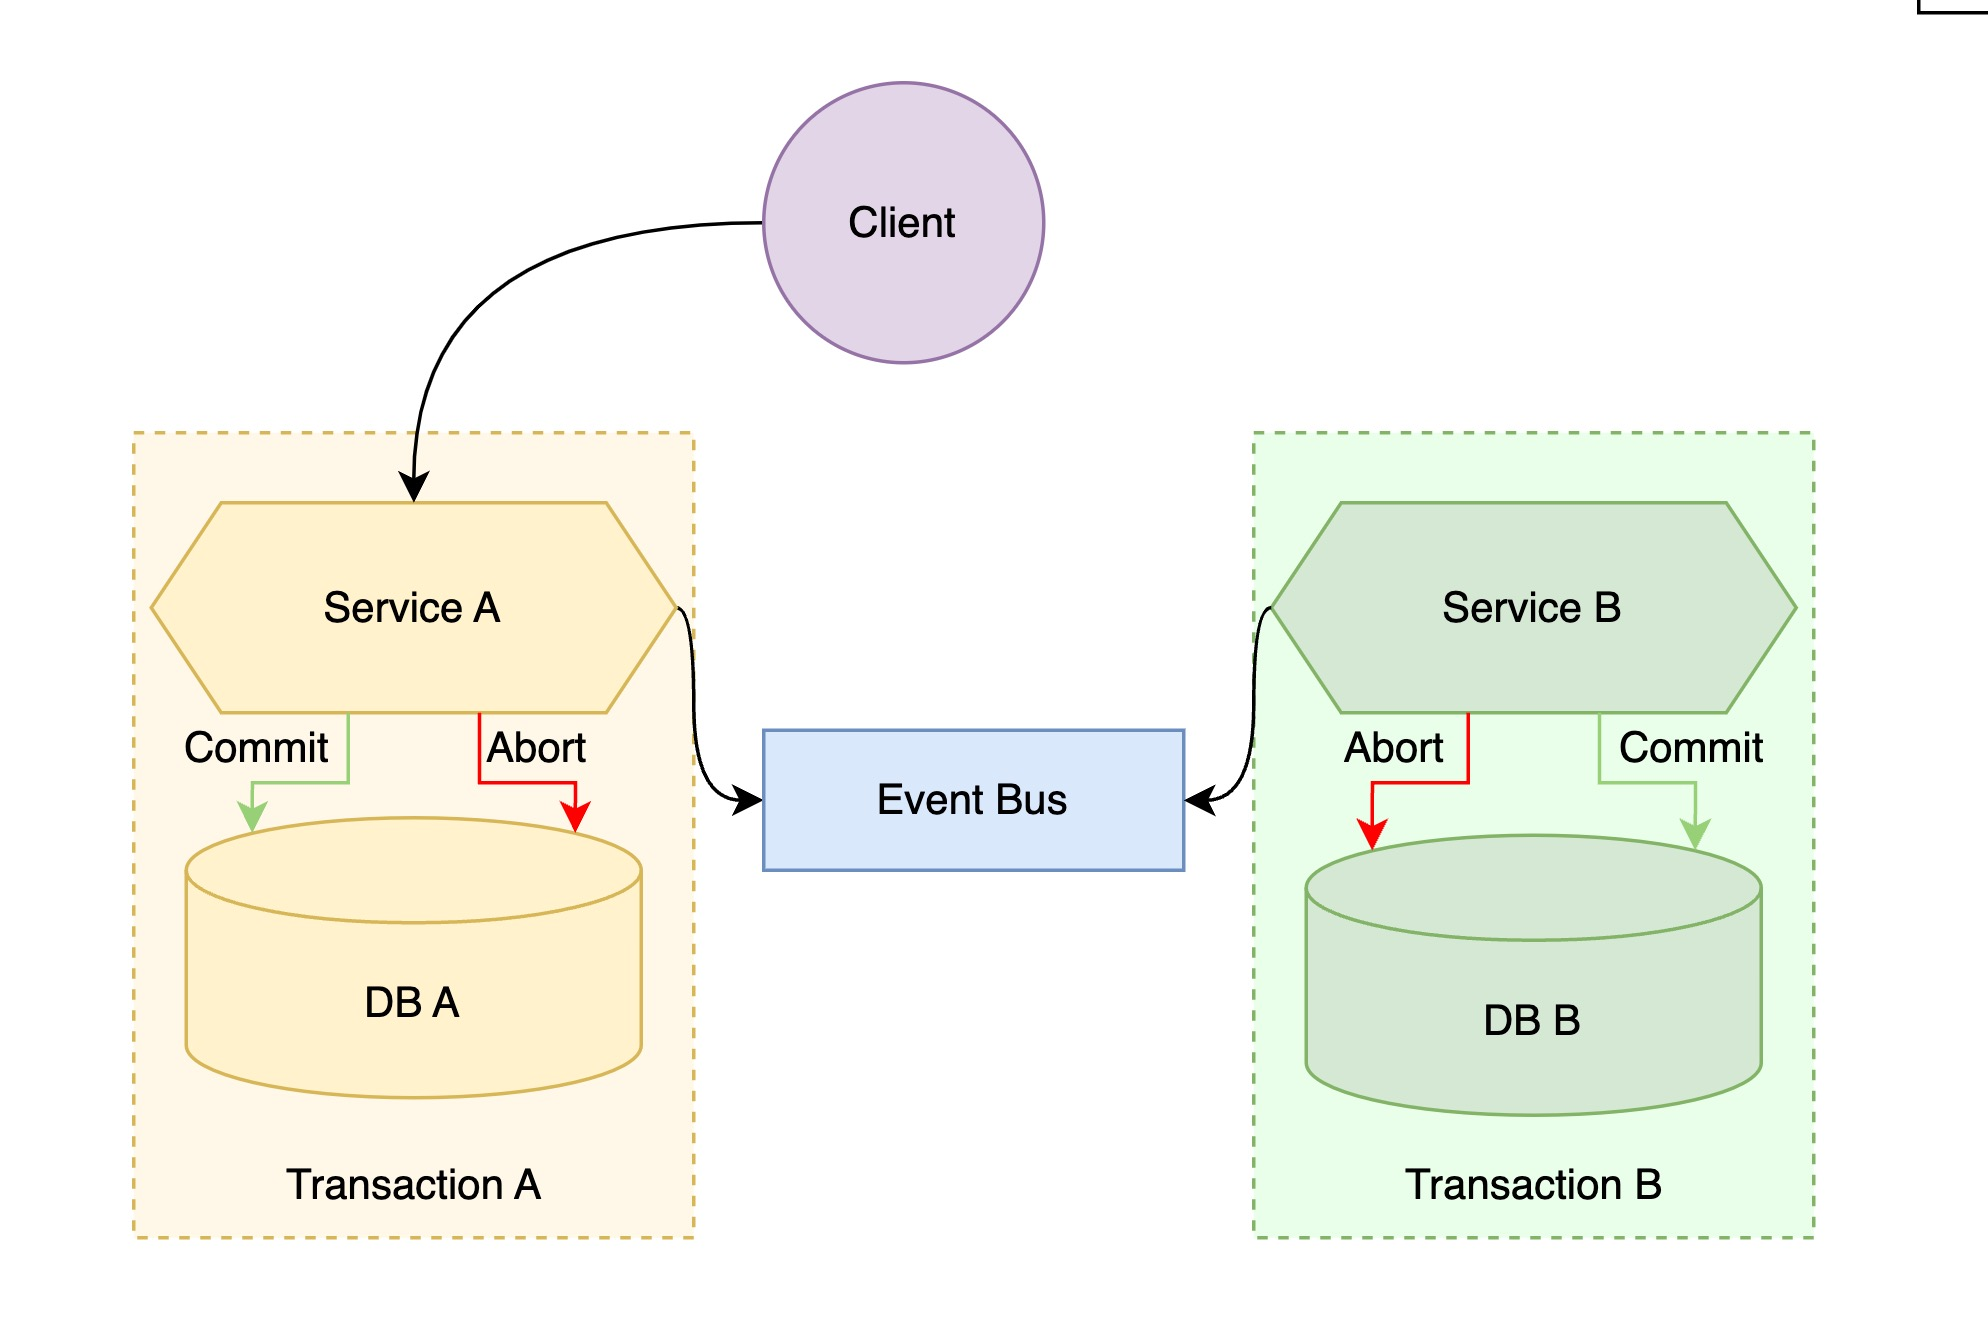
\includegraphics[width=0.8\linewidth]{img/saga_async.jpeg}
    \caption{--- Принцип работы Saga без централизованного координатора}
    \label{fig:saga_async}
\end{figure}

Поэтому иногда коммуникацию между сервисами осуществляют непосредственно через одну из баз данных, которую в асинхронном режиме
сканируют другие сервисы. Постоянное чтение всех данных в базе данных координаторе может вызвать проблемы с производительностью, поэтому 
стоит прибегать к механизмам потоков изменений, как например в YDB. Тем не менее, как было описано ранее, общий доступ в одну базу данных
считается антипатерном при разработке распределенных систем, поэтому не является рекомендуемым подходом.

\begin{figure}[H]
    \centering
    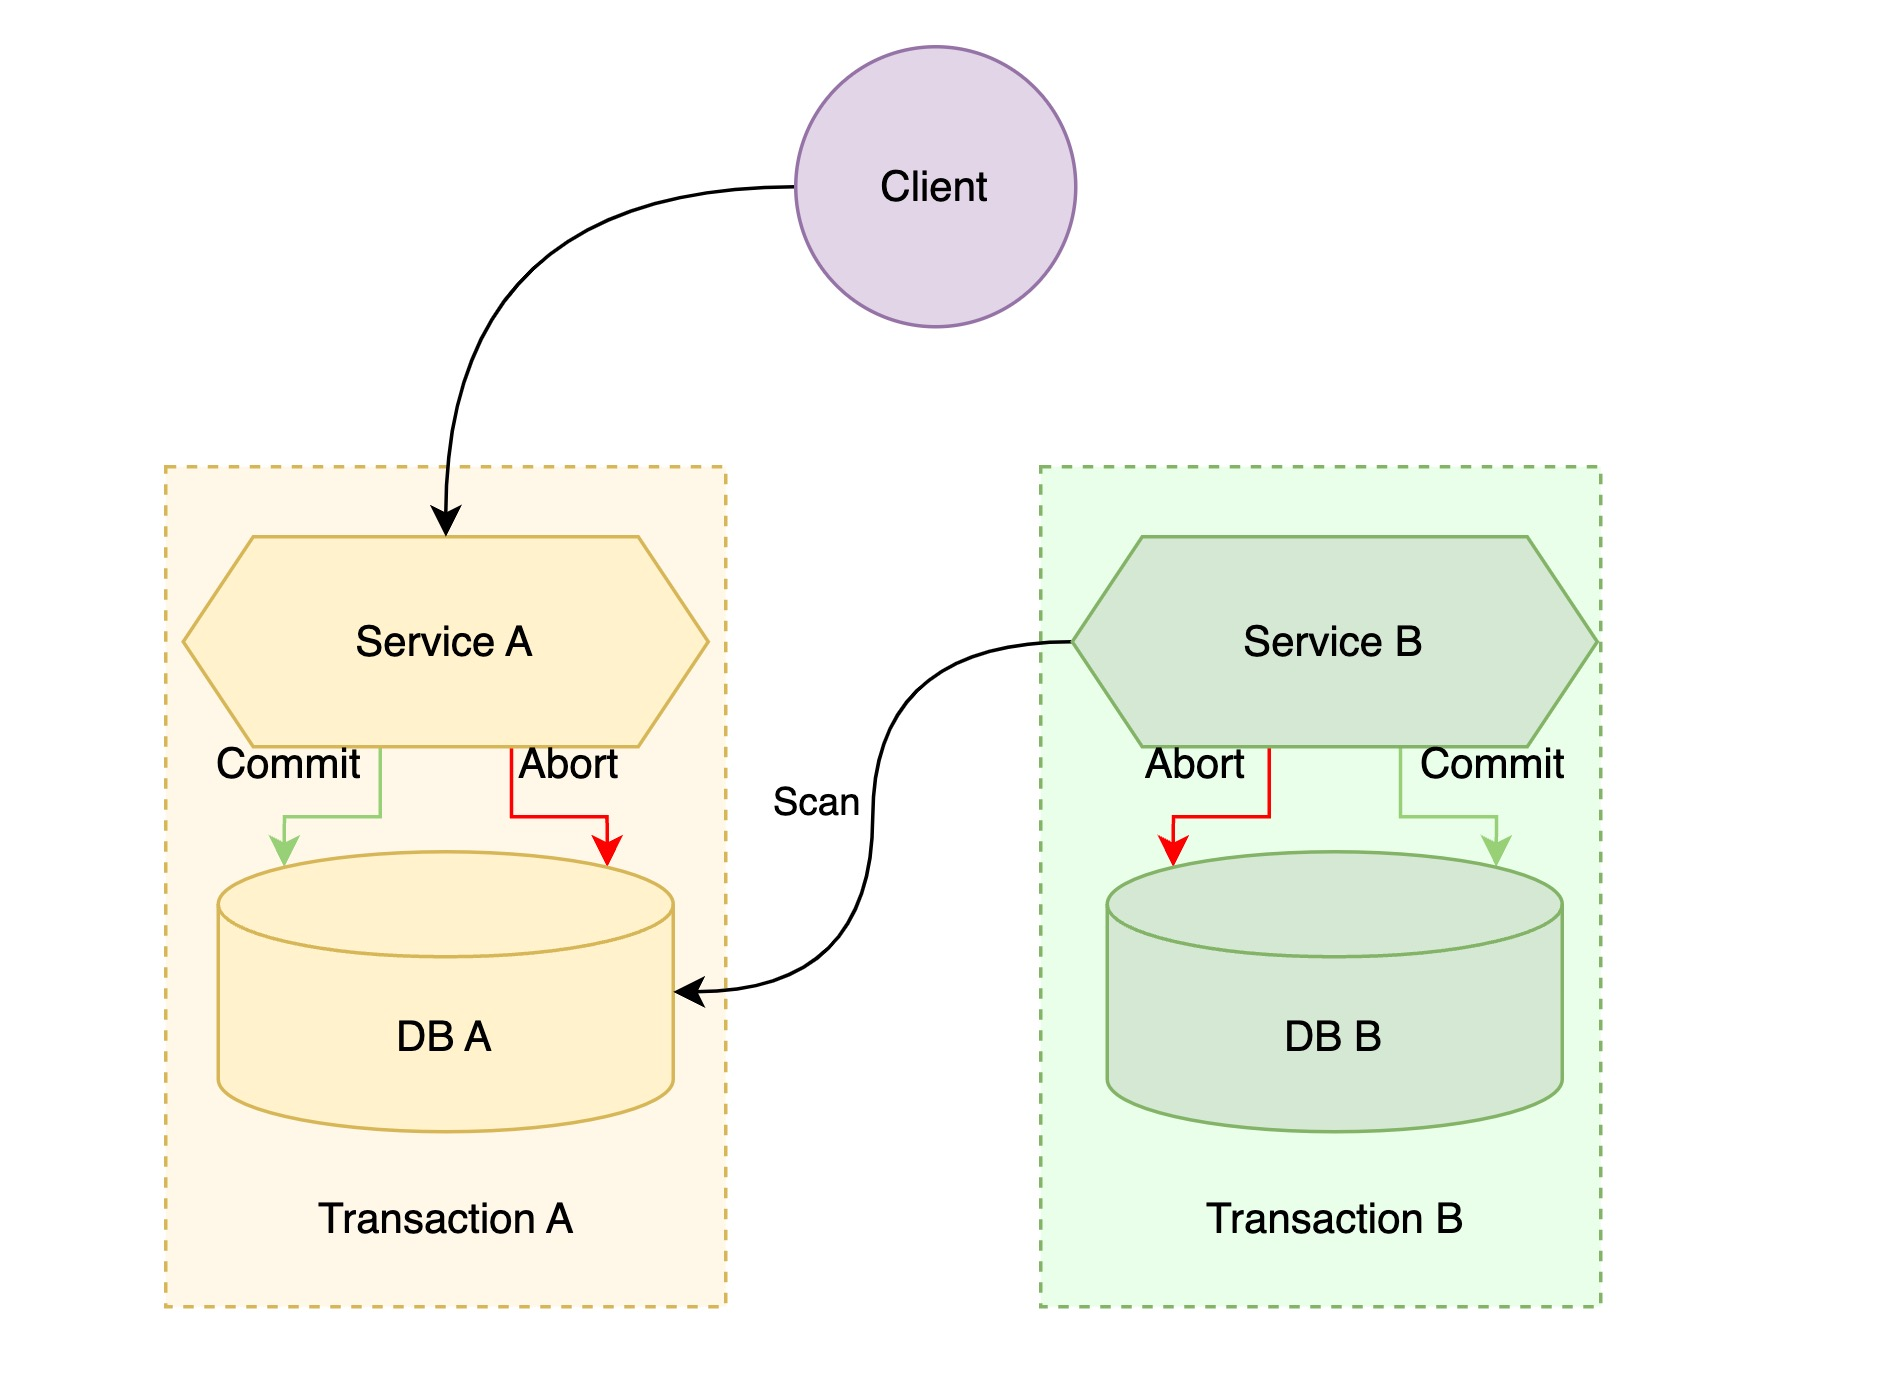
\includegraphics[width=0.8\linewidth]{img/saga_scan.jpeg}
    \caption{--- Принцип работы Saga с синхронизацией через одну из баз данных}
    \label{fig:saga_db}
\end{figure}

\section{Практики применения систем оркестрации в микросервисных архитектурах}
Внедрение микросервисной архитектуры также сопровождается вопросами релизного цикла и выкладки новых версий. Не всегда отдельные компоненты 
системы можно обновлять независимо, тогда как монолитные приложения можно обновлять без дополнительной координации, поскольку вся
система функционирует в рамках одного процесса. Поэтому при внедрении микросервисов стоит обратить особое внимание на системы оркестрации
и непрерывного деплоя, также называемого Green-blue деплоем. 

Green-blue деплой подразумевает совокупность стратегий по постепенной выкатке нового функционала. Одной из
самых распространенных систем оркестрации является Kubernetes, разработанный компанией Google.

Конкретно green-blue деплой реализуется через одномоментное переключение трафика из старых версий веб-приложения
в новые версии (Рисунок \ref{fig:gb}). Быстрое переключение трафика достигается за счет инструментов виртуализации, например, с помощью Docker-контейнеров,
которые содержат образ операционной системы, персистентное переиспользуемое хранилище данных из файловой системы и агенты виртуализации, которые
поддерживают связь с супервизором, который связывает контейнеры с io хостовой операционной системы.
Помимо быстрого переключения на новую версию приложения обеспечивается также возможность быстро откатить
примененные изменения, что является мощным средством предотвращения проблем, связанных с уязвимостями и багами
системы. 
\begin{figure}[H]
    \centering
    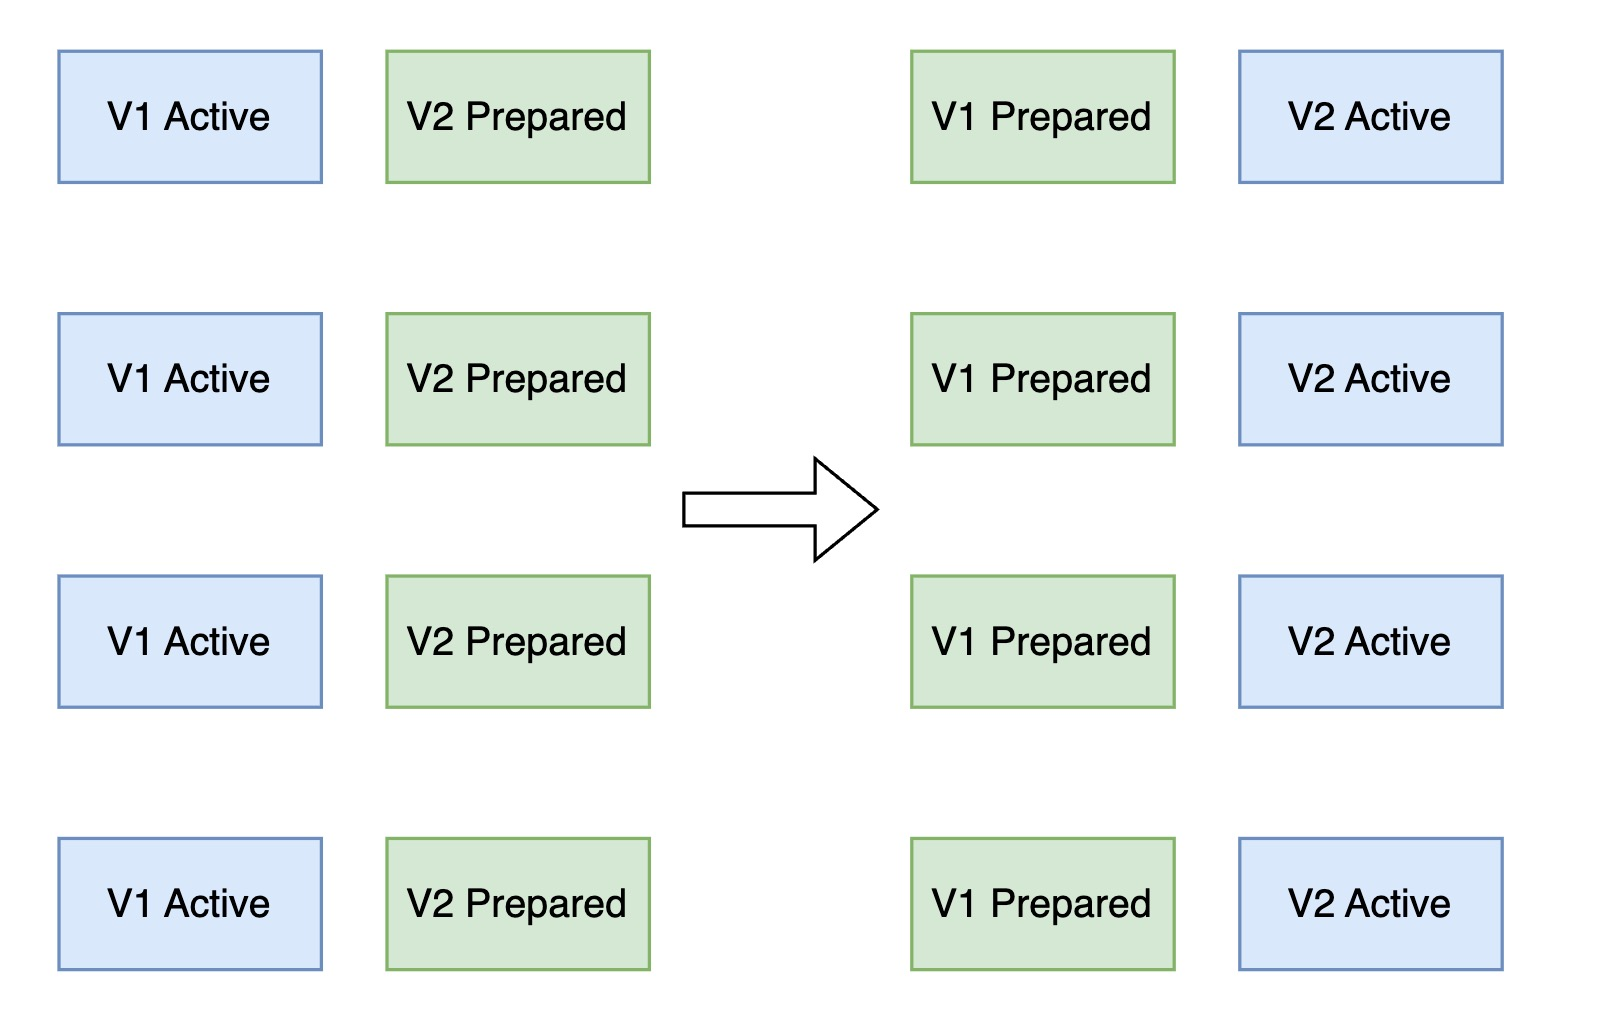
\includegraphics[width=0.8\linewidth]{img/gb.jpg}
    \caption{--- Процесс выкладки при green-blue развертывании}
    \label{fig:gb}
\end{figure}

Помимо green-blue деплоя применяются подходы, вроде rolling обновлений (Рисунок \ref{fig:rolling}), при которых обновление не происходит
одномоментно, а постепенно. В этом случае новая версия приложения также подготавливается заранее, и процесс обновления
постепенно переключает трафик со старых версий на новые.

\begin{figure}[H]
    \centering
    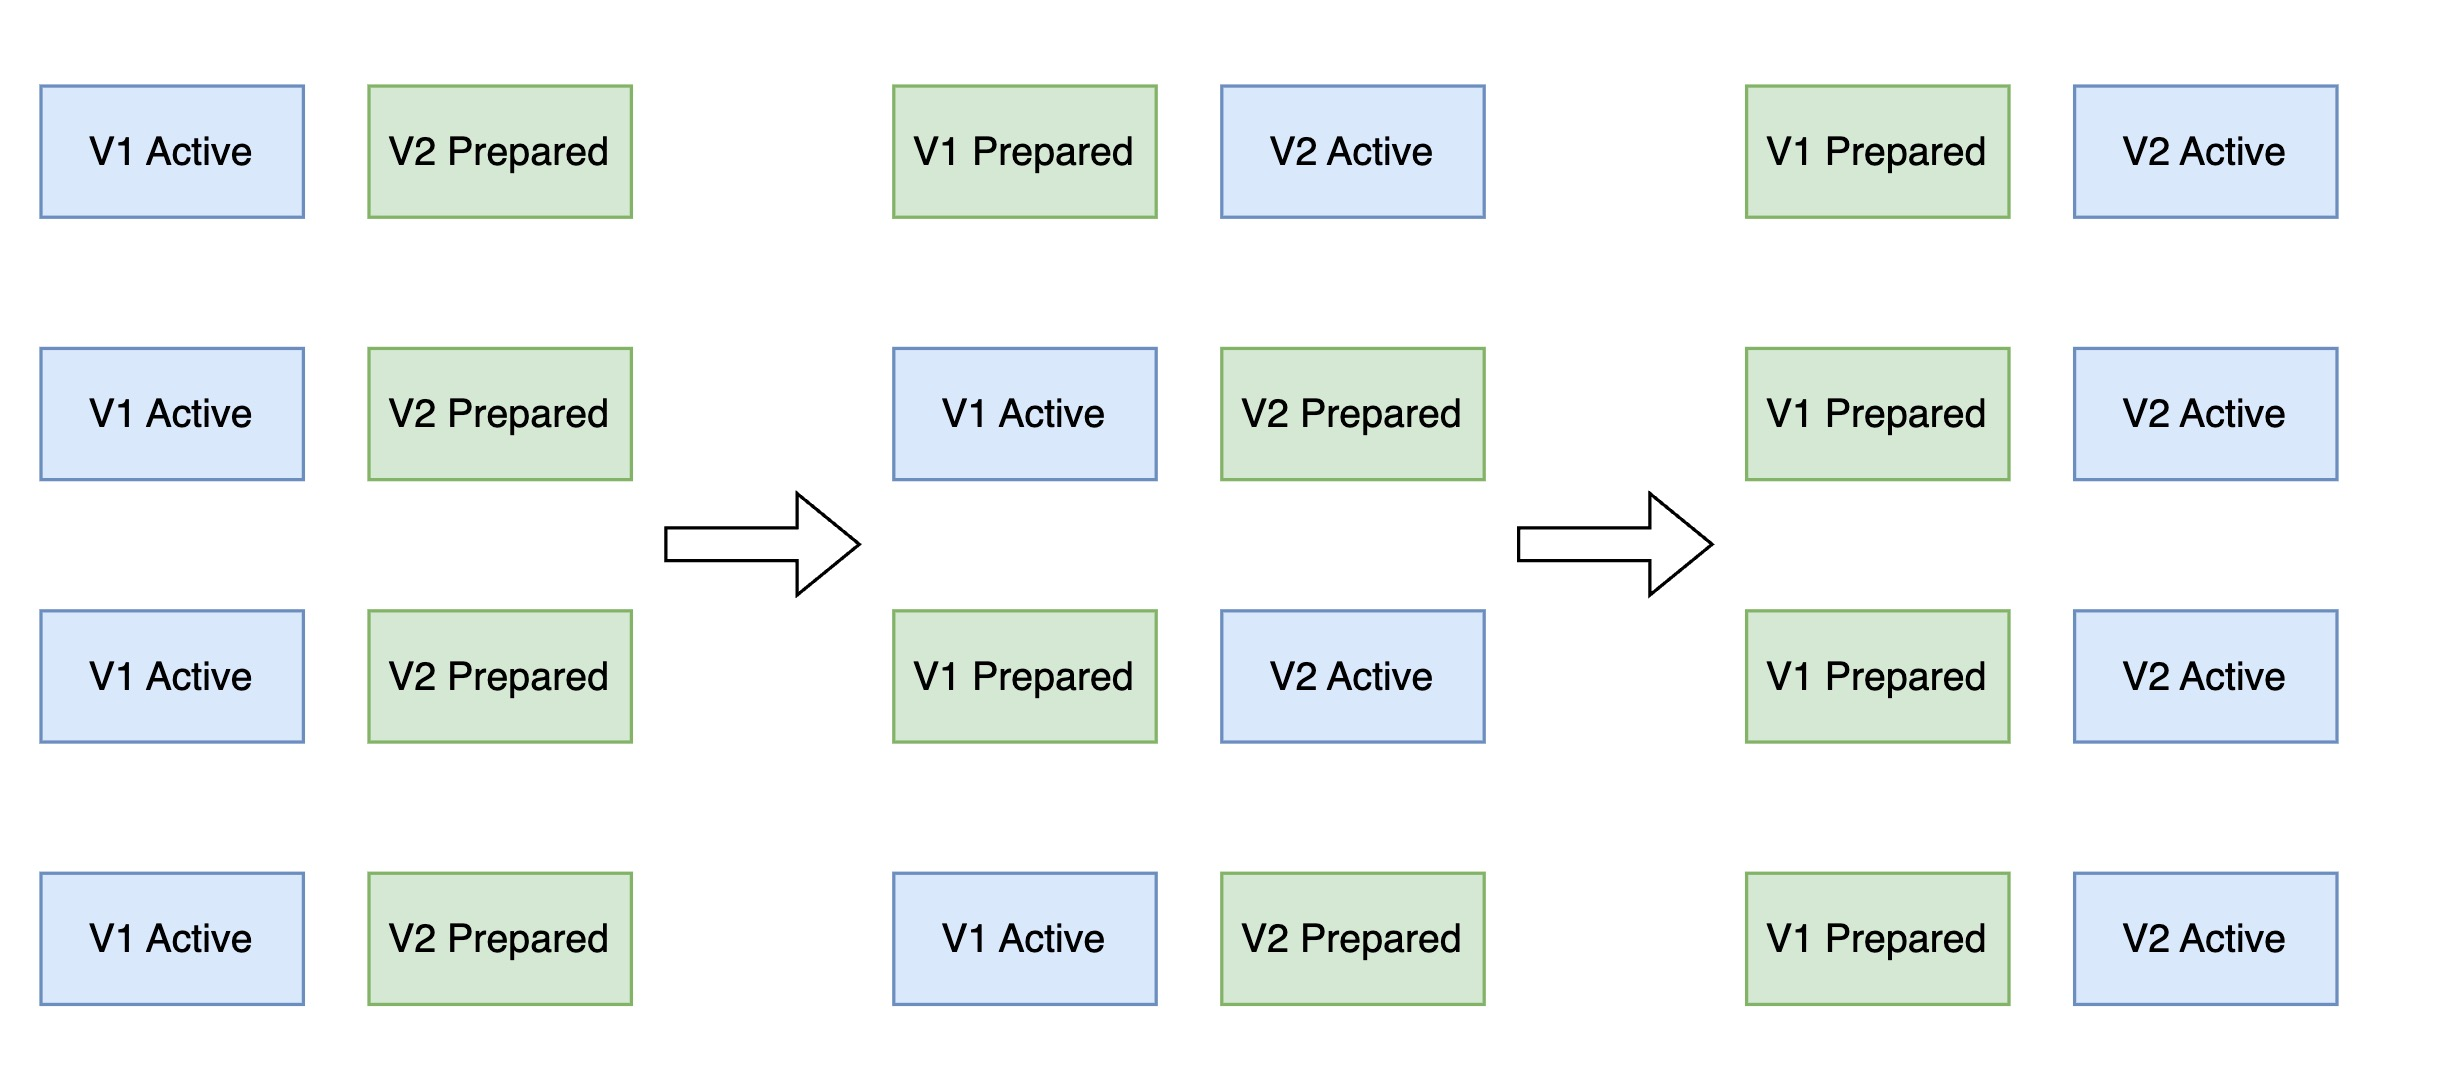
\includegraphics[width=0.8\linewidth]{img/rolling.jpg}
    \caption{--- Процесс выкладки при rolling развертывании}
    \label{fig:rolling}
\end{figure}

Для ранней диагностики проблем также может быть подготовлено отдельное окружение, называемое Canary или престабильным, которое дублирует или делит 
зависимости со стабильной версией, куда будет перенаправляться небольшой процент трафика от случайно выбранных или выбранных
по определенному признаку пользователей (Рисунок \ref{fig:canary}). Подобный подход зачастую применяется крупными компаниями, типа Netflix или Google, для
тестирования нового функционала на пользователях, что значительно упрощает последующую выкладку в стабильное окружение
и минимизирует риски. В подобном подходе помимо систем оркестрации требуется настройка 
сети на балансере прикладного уровня, который будет перенаправлять трафик Canary контур. 

\begin{figure}[H]
    \centering
    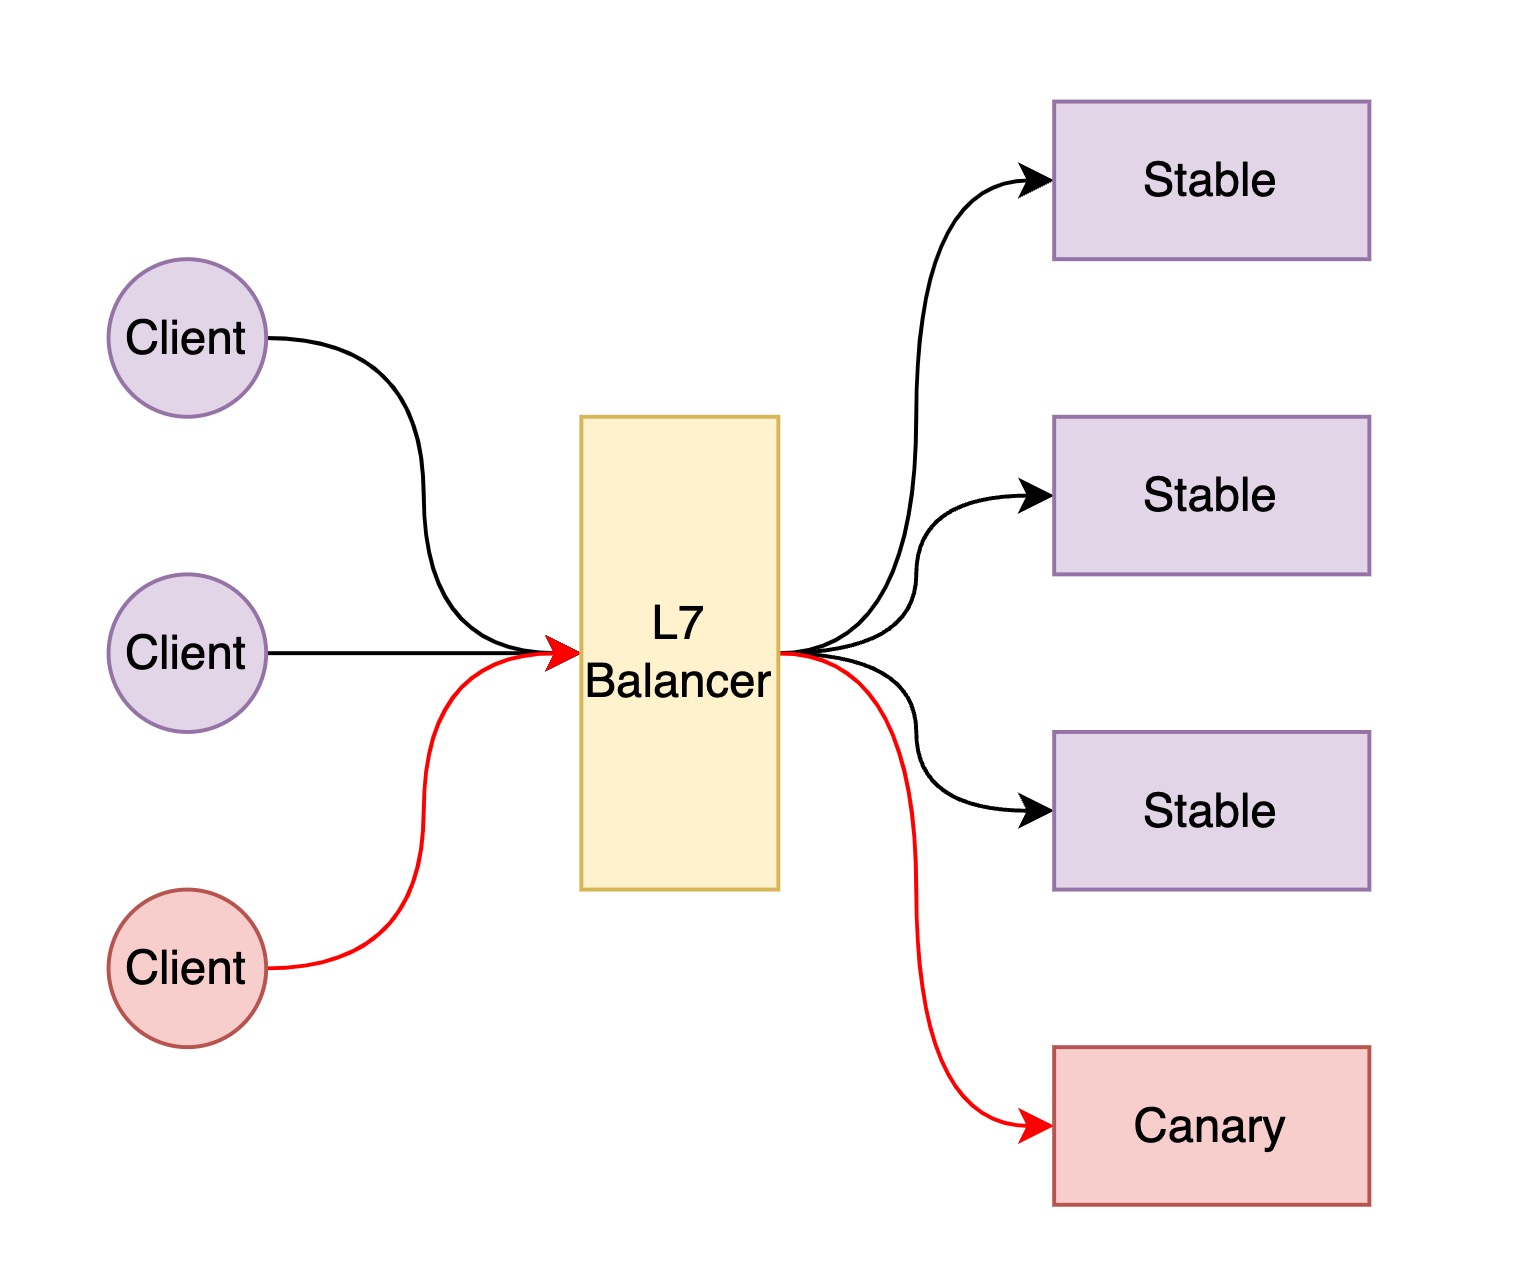
\includegraphics[width=0.8\linewidth]{img/canary.jpg}
    \caption{---  Процесс развертывания c Canary контуром}
    \label{fig:canary}
\end{figure}

Поднятие отдельного окружения может быть дорогостоящим инфраструктурным решением из-за необходимости
выделять ресурсы под отдельные экземпляры приложения. Поэтому аналогичная стратегия может быть
реализована через AB-тестирование или feature-флаги, которое предполагает разделение
пользователей на непересекающиеся группы, для которых будет доступен новый функционал или новое поведение,
скрытое на уровне приложения в стабильной версии. В этом случае учитываются некоторые данные,
которые могут помочь идентифицировать пользователя и передать в виде метаинформации нужные флаги
для активации новой функциональности (Рисунок \ref{fig:ab}). В этом случае тестирование новых версий можно производить более плавно, без
привязки к хостам, содержащим экземпляры приложений, и предоставляет данные для будущей
аналитики, которая может помочь принять решение о целесообразности нововведений.

\begin{figure}[H]
    \centering
    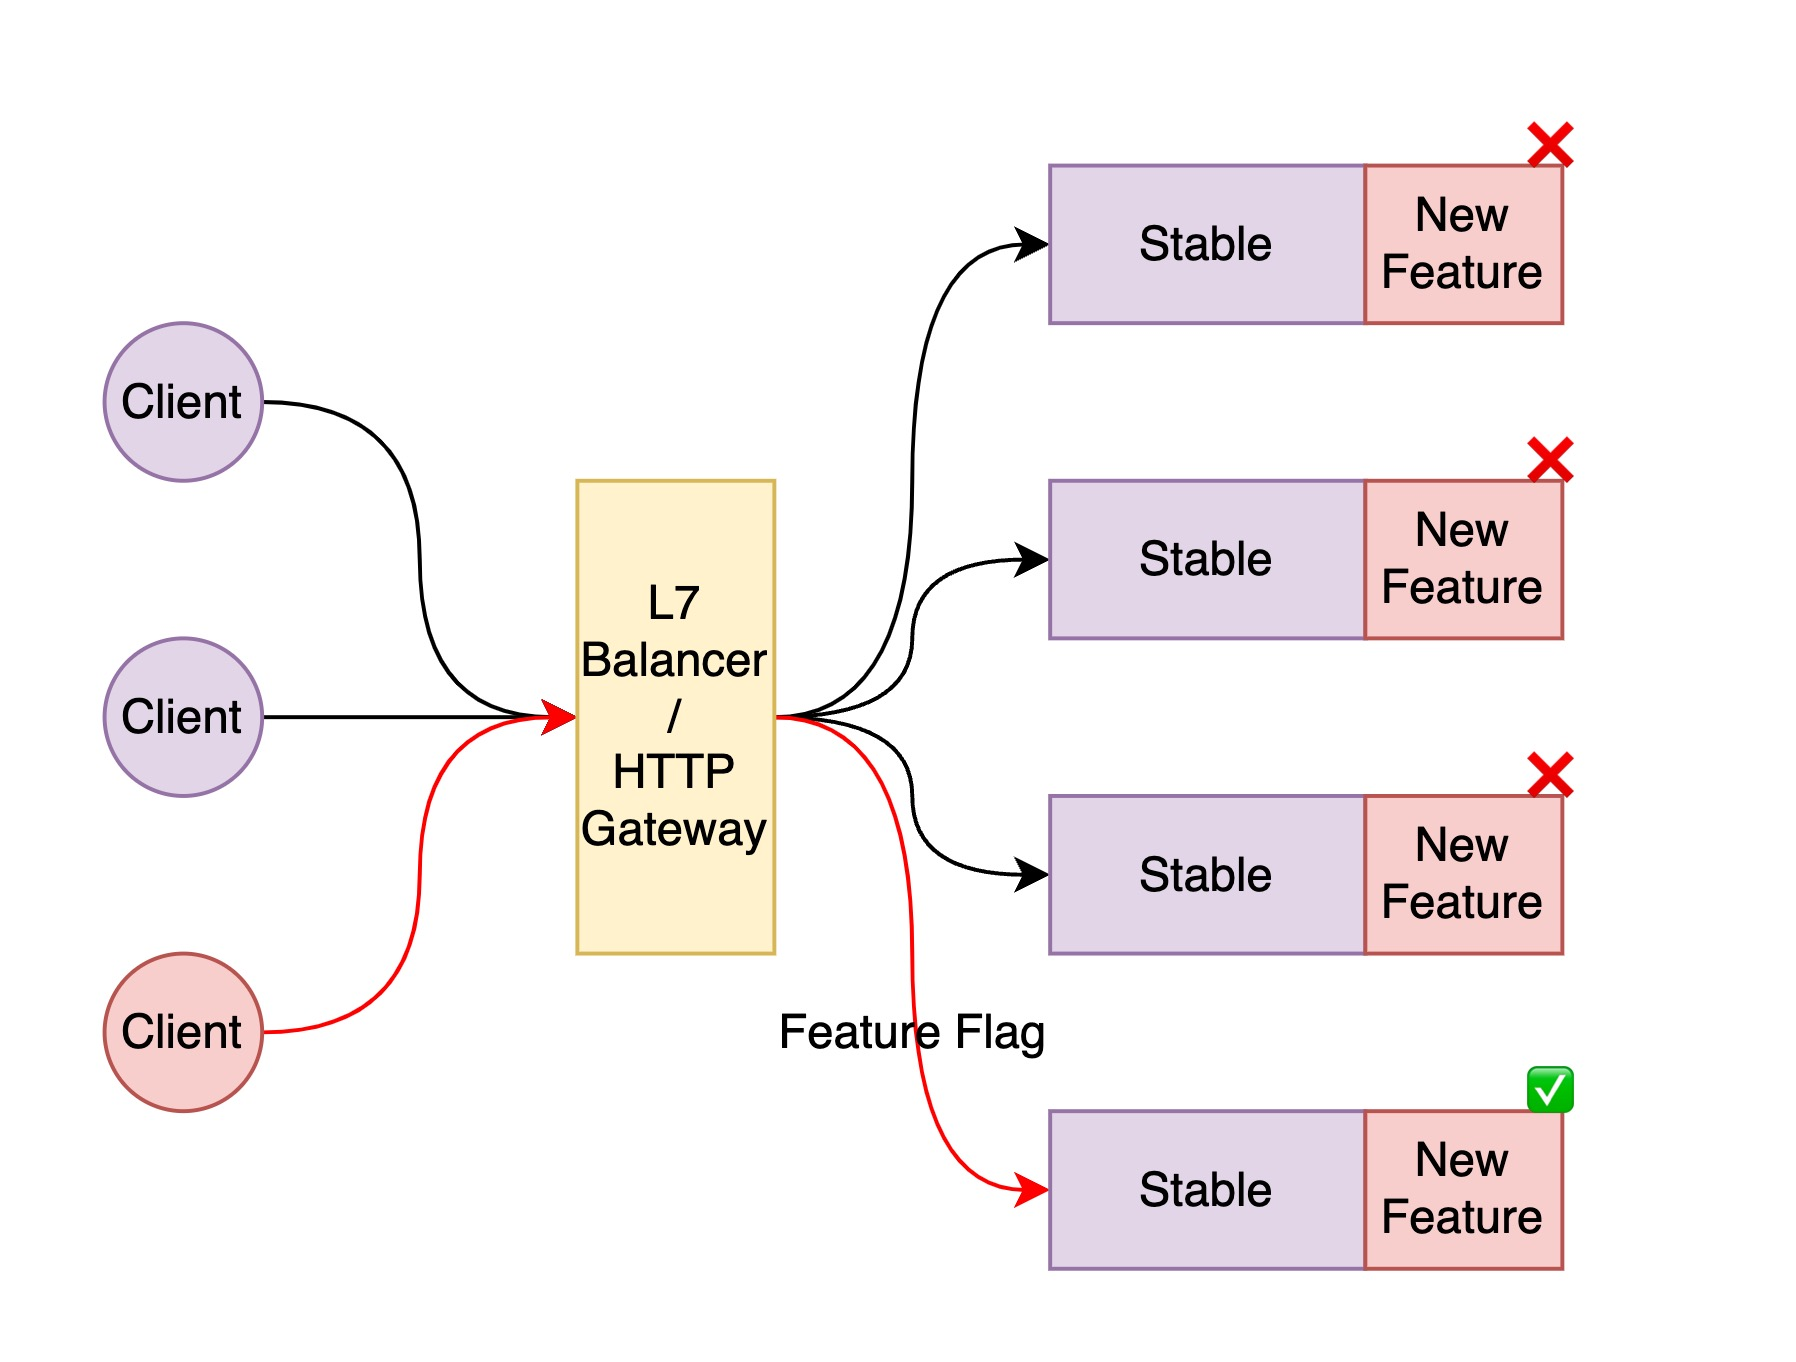
\includegraphics[width=0.8\linewidth]{img/ab.jpg}
    \caption{--- Принцип AB-тестирования}
    \label{fig:ab}
\end{figure}

В рамках тестирования новой функциональности применяется также sha\-dow deployment или теневые выкладки,
при которых трафик в стабильные версии зеркалируется в отдельные экземпляры приложения со своими персистентными хранилищами,
которые могут быть воспроизведены из оригинальных данных, что помогает оценить отказоустойчивость
приложения под нагрузкой или провести инструментацию сервиса без вреда производительности (Рисунок \ref{fig:shadow}).
Примером инструментации, которая может нести в себе потенциальные проблемы с производительностью
является PGO (Profiler Guided Optimisation), который предполагает сбор широкого спектра данных о
процессорном времени, аллокации памяти, состояния рантайма и так далее, что требует накладных расходов.
Полученные данные в последующем могут быть использованы при сборке приложения для выявления сценариев
использования системы, что подсказывает компилятору, какие оптимизации можно применить.
Сбор данных о производительности приложения в отдельном контуре может помочь наладить подобный процесс, не замедляя
при этом стабильные версии приложения.
\begin{figure}[H]
    \centering
    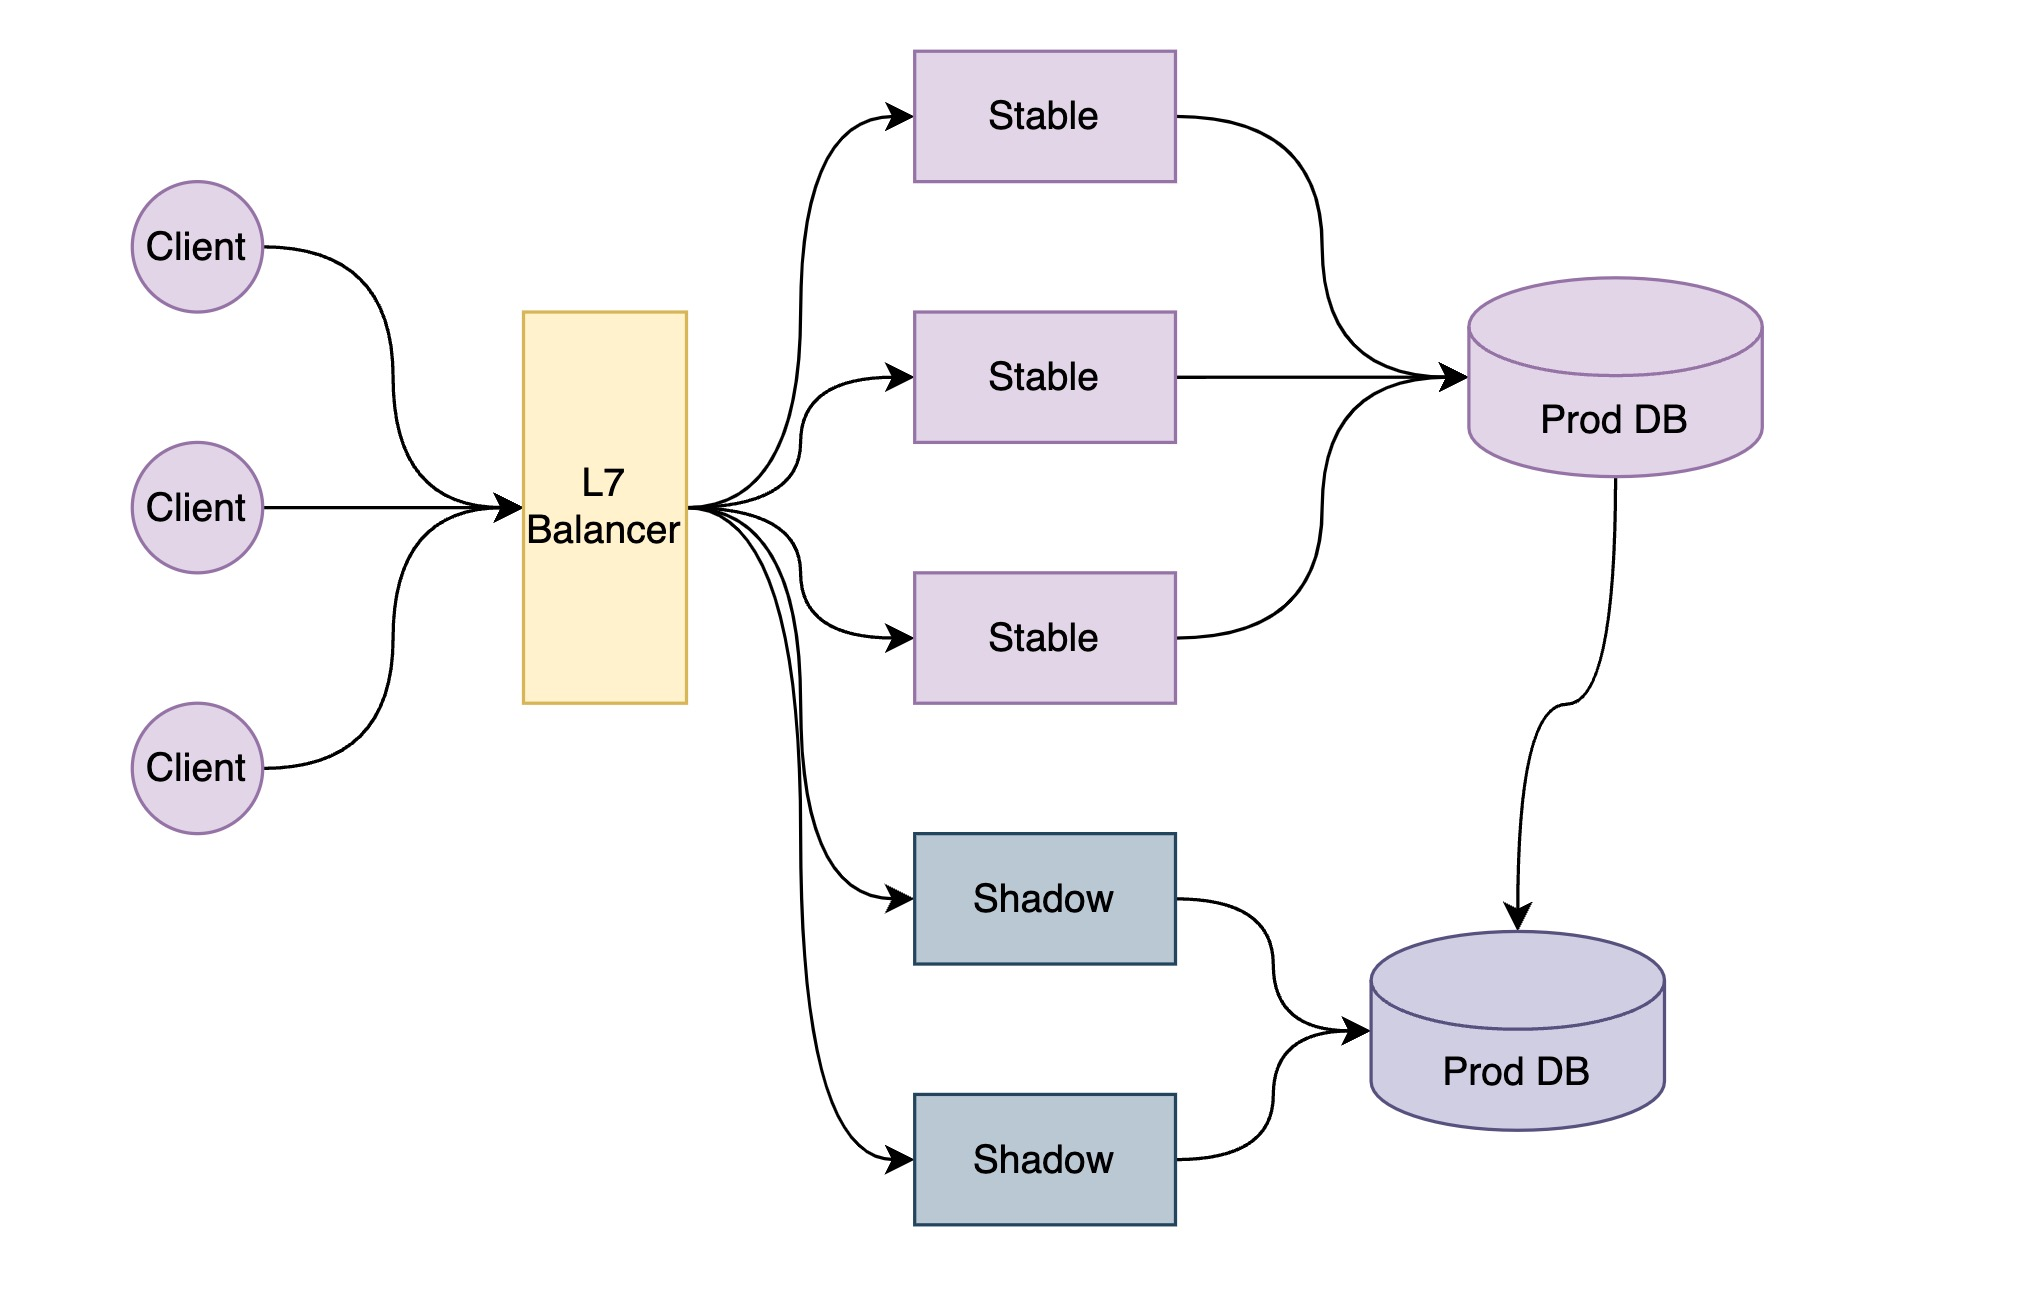
\includegraphics[width=0.8\linewidth]{img/shadow.jpg}
    \caption{--- Принцип зеркалирования трафика при shadow развертывании}
    \label{fig:shadow}
\end{figure}

В этом случае изменения можно выпускать бесперебойно и с учетом нескольких зон
доступности, что позволяет проводить инструментацию и мониторинг сервиса на самих ранних стадиях релизного цикла.
Несмотря на вышеперечисленные проблемы, при правильном проектировании микросервисной архитектуры и применении правильных сетевых и практик оркестрации 
релизы микросервисов могут быть проще релизов монолитных приложений, поскольку можно выкатывать функциональность независимо от других 
сервисов, что упрощает тестирование и позволяет иметь отдельный релизный цикл.

Еще одна трудность связана с решением о том, на каком этапе жизненного цикла
приложения следует переходить на микросервисную архитектуру. Часто во время
разработки первой версии система не сталкивается с проблемами, которые эта
архитектура решает \cite{kaban}. 

Более того, применение сложного, распределенного метода
проектирования замедлит разработку. Для небольших команд, которым обычно важнее всего
как можно быстрее развивать свою бизнес-модель и сопутствующее приложение, это
может вылиться в непростую дилемму. Использование микросервисной архитектуры делает выпуск начальных версий довольно трудным. Маленьким проектам почти всегда
лучше начинать с монолитного приложения.

Однако со временем возникает другая проблема: как справиться с возрастающей сложностью. Это подходящий момент для того, чтобы разбить приложение
на микросервисы с разными функциями. Рефакторинг может оказаться непростым
из-за запутанных зависимостей. В связи с этим к переходу на них следует отнестись очень серьезно. Но обычно для сложных проектов, таких как пользовательские веб- или
SaaS-приложения, это правильный выбор. Такие общеизвестные сайты, как eBay, Amazon.com, Groupon и Gilt, в свое время перешли на микросервисы с монолитной архитектуры.

При использовании микросервисов приходится иметь дело с множеством проблем, связанных с проектированием и архитектурой.
К тому же многие из этих
проблем имеют несколько решений со своими плюсами и минусами. Единого
идеального решения не существует \cite{micro-1}.

Также IDE и другие инструменты разработки рассчитаны на создание монолитных
приложений и не обеспечивают явной поддержки распределенных приложений. Зачастую микросервисы живут в разных репозиториях, что
требует отдельного версионирования каждого из компонентов. Для решения подобных проблем в некоторых системах сборки прибегают к использованию
воркспейсов, где исходные коды общего кода берутся вне зависимости от релизного цикла микросервисов, а из локальной версии репозитория,
что может облегчить локальную разработку. Однако не всегда разные микросервисы размещаются в разных репозиториях и возникает вопрос
масштабирования инфраструктуры для сборки, тестирования и разработки всего приложения. Репозитории с большим количеством независимых сервисов, но
общими версиями внешних зависимостей зачастую называют монорепозиториями. В монорепозитории инструменты сборки не всегда работают оптимально
без дополнительной конфигурации и эвристик, направленных на кэширование артефактов сборки, однако данные недостатки сопровождаются потенциальными
достоинствами в виде переиспользования кода, повышенной безопасности за счет централизации зависимостей.


\section{gRPC в разработке микросервисов}

Как уже было упомянуто в предыдущем пункте, обмен данными между микросервисами имеет большое значение при проектировании распределенных систем. При правильном проектировании микросервисы сохранят свою
автономность, в то же время необходимо вносить в них изменения и выпускать их новые версии независимо от остальных частей системы. При некорректном исполнении система будет функционировать со сбоями и низкой производительностью, что недопустимо при построении микросервисной архитектуры.

Для определения способа взаимодействия одного микросервиса с другим имеется
выбор между текстовыми форматами данных, как JSON, XML, SOAP и т.д, и бинарными форматами данных такими, как Protocol Buffers, Flatbuffers, 
Cap'n Proto и Simple Binary Encoding. 

При выборе формата передачи данных обычно руководствуются скоростью сериализации и десериализации, простотой использования и поддержкой со стороны сообщества и разработчиков.

Текстовые форматы данных обычно лучше всего поддержаны инструментами разработки и не требуют дополнительных усилий по внедрению их в API сервисов, однако они значительно проигрывают в скорости передачи данных и не предоставляют возможности версионирования без runtime проверок схемы данных, что несет еще большие накладные расходы при конвертации данных, несмотря на то, что за время своего существования парсеры для данных форматов, в частности JSON и XML, были сильно оптимизированы и поддержаны виртуальными машинами многих языков. Поэтому при выборе формата данных для коммуникации микросервисов обычно выбирают бинарные форматы с возможностью версионирования и строгой схемой \cite{Bolanowski_2022}.

Вышеупомянутые Cap'n Proto, SBE и Flatbuffers демонстрируют хорошую производительность в синтетических тестах, однако не обладают поддержкой широкого списка языков программирования и инструментов для разработки \cite{comp}. Protocol Buffers же предлагает разумный компромисс между производительностью и простотой использования, поэтому в настоящий момент является самым популярным вариантом при разработке микросервисов \cite{protobuf}.

Для написания Protobuf файлов используют язык описания интерфейсов (IDL).
Например, чтобы описать структуру данных сообщения, нужно добавить message, имя структуры, а внутри тип, название и номер поля. Номера полей нужны для обратной совместимости, поэтому не стоит менять их последовательность при добавлении или удалении полей. Образец сообщения представлен в листинге \ref{lst:proto}.
\begin{lstlisting}[caption={Сетевые хендлеры, осуществляющие основую логику},label=lst:proto,captionpos=b] 
syntax = "proto3";
package user;

service User {
  rpc GetUser(GetUserRequest) returns (UserInfo) {}
  rpc CreateUser(UserInfo) returns (UserStatus) {}
}

message UserInfo {
  string email = 2;
  string name = 3;
  repeated string phone = 4;

  message Address {
    string street = 1;
    string city = 2;
    string state = 3;
    string zip = 4;
  }

  Address address = 5;
}

message GetUserRequest {
  string email = 1;
}

message UserStatus {
  string error = 1;
}
\end{lstlisting}


В Protocol Buffers данные представлены и передаются в
бинарном формате, что существенно уменьшает время сериализации/десериализации
данных. Также с применением механизма Protocol Buffers размер передаваемых данных в разы меньше \cite{Bolanowski_2022}.

В настоящее время наиболее популярным RPC-решением для интеграции
микросервисов является gRPC, который по умолчанию использует Protocol Buffers для кодирования сообщений. Это высокопроизводительный фреймворк, разработанный компанией Google для вызовов удаленных процедур, работающий поверх протокола
HTTP/2. Как и во многих RPC-системах, gRPC основан на идее определения сервиса,
указывающий методы, которые можно вызвать удаленно с их параметрами и
возвращаемыми типами \cite{grpc}.

На стороне сервера реализуются методы, которые предоставляются для клиентов, и
запускается gRPC-сервер для обработки клиентских запросов. На стороне клиента
используется заглушка, которая предоставляет те же методы, что и сервер. Его высокая производительность достигается за счет использования протокола HTTP/2 и Protocol Buffers.

Однако у gRPC есть ряд недостатков, которые стоит учитывать при проектировании систем с применением данной технологии. Во-первых, Protocol Buffers это бинарный формат, поэтому для отладки и разработки приложений требуется иметь актуальную версию схемы данных, что делает невозможным отправку с клиента произвольных запросов и затрудняет отладки вне слоя приложения, где данные не представлены человекочитаемым форматом. Во-вторых, несмотря на то, что в 2022 была представлена спецификация протокола HTTP/3, HTTP/2 все еще имеет ограниченную поддержку со стороны браузеров, что делает невозможным непосредственную коммуникацию между веб-клиентом и сервисами. 

Частично это проблема решается специальными расширениями, которые добавляют HTTP-прокси слой, который проксирует HTTP/1 запросы с небинарным форматом данных, например, JSON, в HTTP/2 запросы с данными в формате Protocol Buffers, однако это нивелирует достоинства бинарной сериализации из-за необходимости дополнительной конвертации данных между форматами.

Поэтому при проектировке систем общеиспользуемый REST API интерфейс присутствует лишь во внешнем слое приложения и может быть реализован без расширений, исходя из конкретной бизнес-логики, что добавляет накладные расходы на цикл сериализации и десериализации лишь во входном и выходном запросах.
\section{Обзор языка программирования Golang }
Go (также известный как Golang) является статически типизированным компилируемым языком программирования, разработанным на замену ранним языкам системного программирования, таким как C\textsuperscript{++} и Java. 
Созданный Google, Go предоставляет упрощенный синтаксис и мощные инструменты для разработки операционных систем, сетевых сервисов, микросервисов и других распределенных систем \cite{golang}.

Для простоты внедрения данного языка было уделено большое внимание простоте синтаксиса и грамматике языка. 
Многие задачи имеют лишь одно решение средствами языка Go, которое описывается общеизвестными методами парадигм ООП и структурного программирования. 
За счет просты грамматики также достигается высокая скорость компиляции, что положительно сказывается на опыте разработки.

Также для устранения факторов, мешающих разработке, в стандартной поставке языка также предусмотрены инструменты для управления зависимостями и сборки, форматирования кода, синтаксического анализа, генерации и просмотра документации, а также профилирования готовых приложений.

Несмотря на то, что исходные коды языка находятся в общем доступе под свободной лицензией,
процесс разработки по большей части контролируется разработчиками Google и многие решения проходят процесс согласования с проектировщиками языка в лице Кена Томпсона, который участвовал в разработке системы UNIX, Роба Пайка, известного за вклад в развитие операционной системы Plan9, и Роберта Гриземера, который до этого работал над виртуальной машиной V8 для языка JavaScript.

Поэтому, с одной стороны, участие сторонних разработчиков над ядром языка ограничено, поэтому новый функционал принимается с большим количеством обсуждений и согласований, за что язык регулярно критикуют.

Есть мнение, что в текущей реализации языка отрицается многолетний опыт разработки других языков, что отражается в использовании очень простой системы типов, сборщика мусора на поколенческом алгоритме и общей невыразительности базовых синтаксических элементов языка .

С другой стороны, подобный подход гарантирует полную обратную совместимость со старыми программами и маленькое ядро языка с выверенным набором инструментов, которые призваны уменьшать количество дискуссий по поводу вопросов, которые не имеют к разработке прямого отношения: сборка, форматирование, дистрибуция. Что в связке с богатой библиотекой для работы с сетевыми стеками делает Golang хорошим выбором при разработке программ, связанных с веб-разработкой, и послужило причиной выбора данного языка в разработке программного обеспечения для данной работы.

\section{Основные инструменты построения распределенных архитектур}
Одним из ключевых вопросов при построении распределенных архитектур является асинхронная коммуникация
между миросервисами, которая позволяет независимо масштабировать ее компоненты.

Брокер сообщений служит критически важным компонентом при проектировании архитектуры микросервисов, работая как посредник при передаче данных между различными сервисами, 
он позволяет минимизировать прямые связи и обеспечивает ряд ключевых преимуществ, которые облегчают разработку, масштабирование и поддержку сложных микросервисных систем.
Одно из основных преимуществ использования брокера сообщений -- возможность полного разделения различных компонентов системы. 
В архитектуре микросервисов подобное разделение является важным фактором в обеспечении независимости каждого из сервисов. 
Благодаря брокеру сообщений, компоненты в системе не должны прямо общаться друг с другом, что повышает их изоляцию и позволяет им работать независимо. 
Это упрощает процесс обновления или модификации отдельных компонентов, поскольку минимизирует риск сбоев всей системы из-за изменений в одном из сервисов.

Далее, использование брокера сообщений увеличивает надежность системы. Благодаря использованию промежуточного слоя для передачи сообщений, они могут быть надежно сохранены и переданы даже при временных сбоях приема или трансляции. 
Это гарантирует, что важные данные не будут потеряны из-за сбоев или проблем с конкретными сервисами, усиливая отказоустойчивость всей системы.

Помимо этого, брокеры сообщений обеспечивают асинхронную передачу данных. 
Это означает, что система не требует немедленного ответа от сервиса-получателя, что может быть критически важно при высоких нагрузках. 
Брокеры сообщений могут агрегировать сообщения и управлять их доставкой оптимальным образом, обеспечивая более плавную и эффективную работу системы.

На рынке представлено множество различных брокеров сообщений, включая RabbitMQ, Apache Kafka, Google Pub/Sub и AWS Simple Queue Service (SQS). 
Каждый из этих продуктов предлагает различные функции и возможности, такие как надежные очереди сообщений, модели публикации/подписки, устойчивость к ошибкам и многое другое. 
Это позволяет разработчикам выбирать наиболее подходящий брокер сообщений для их конкретных нужд и требований.

В итоге, брокеры сообщений играют ключевую роль в архитектуре микросервисов. Они повышают надежность и устойчивость системы, обеспечивают разделение между сервисами и позволяют более эффективно управлять данными и нагрузкой в рамках сложных микросервисных экосистем.

В данной работе основной акцент делается на Amazon Simple Queue Service (SQS), поскольку он является мощным инструментом для обработки сообщений в архитектуре микросервисов и обладает несколькими ключевыми преимуществами, 
которые делают его привлекательным выбором для различных сценариев использования.

Amazon SQS предлагает высокую надежность благодаря инфраструктуре Amazon. 
Сервис гарантирует доставку сообщения хотя бы один раз, что помогает избежать потери данных. Кроме того, Amazon SQS предлагает очереди с повышенной отказоустойчивостью, которые хранят сообщения на протяжении определенного времени, пока они не будут успешно обработаны получателем.

Amazon SQS легко масштабируется, чтобы обеспечивать эффективную обработку больших объемов данных. 
Благодаря возможности бесконечного расширения, этот сервис может гибко настраиваться для поддержки микросервисов любого размера, чтобы поддерживать высокую производительность без дополнительных усилий с вашей стороны.
Также благодаря тесной интеграции с AWS Identity and Access Management (IAM), Amazon SQS позволяет точно контролировать доступ к очередям сообщений, обеспечивая высокий уровень безопасности. Также доступны функции транзитного шифрования для дополнительной защиты данных.

Вместе с облачной инфраструктурой предоставляются SDK для разных языков, включая AWS Management Console, SDK и CLI. Что позволяет использовать одинаковые семантики и метод API вне зависимости от языка и освобождает от необходимости писать свои клиенты для
взаимодействия с очередью.
Также если вы уже используете другие сервисы от AWS, такие как Lambda, S3 или EC2, использование SQS значительно упрощает интеграцию микросервисов, поскольку все они работают вместе без каких-либо существенных проблем. Использование
S3, например, в качестве промежуточного медиума может позволить передавать сообщения большого размера вне зависимости от отграничений SQS, что представлено в Java SDK для работы с SQS.

Таким образом, Amazon SQS представляет собой отличный выбор для обработки сообщений в архитектуре микросервисов благодаря своей надежности, масштабируемости, безопасности и простоте использования. Благодаря настройке под конкретные потребности и легкой интеграции с другими сервисами AWS, SQS может стать очень ценным активом в микросервисной архитектуре.

При локальной разработке необязательно прибегать к выделению облачных инстансов SQS, а можно воспользоваться сторонними реализациями, которые доступны для развертывания вне облачной инфраструктуры AWS. Примерами подобных решений являются Localstack, Minio, а также официальные образы Amazon
некоторых сервисов, доступных в облаке.

В контексте реализации асинхронного взаимодействия между микросервисами применяются следующий набор методов SDK для языка Go:
\begin{enumerate}
    \item SendMessageWithContext, который отправляет закодированное сообщение в произвольном формате в очередь с адресом QueueUrl и позволяет отменять вызов низлежащего сетевого запроса по переданному Context.
    \item ReceiveMessageWithContext, который получает MaxNumberOfMessages сообщений из очереди с адресом QueueUrl и так же предоставляет синхронизацию через Context.
    Чтение данным методом автоматически проставляет период видимости сообщений, при котором сообщения не будут прочитаны другими 
    потребителями повторно.
    \item DeleteMessageWithContext, который окончательно удаляет сообщение из очереди адресом QueueUrl, а также предоставляет синхронизацию через Context.
     Данный метод реализует подтверждение обработки сообщения и в других 
    брокерах может называться Acknowledge (ACK).
\end{enumerate}

\begin{figure}[H]
  \centering
  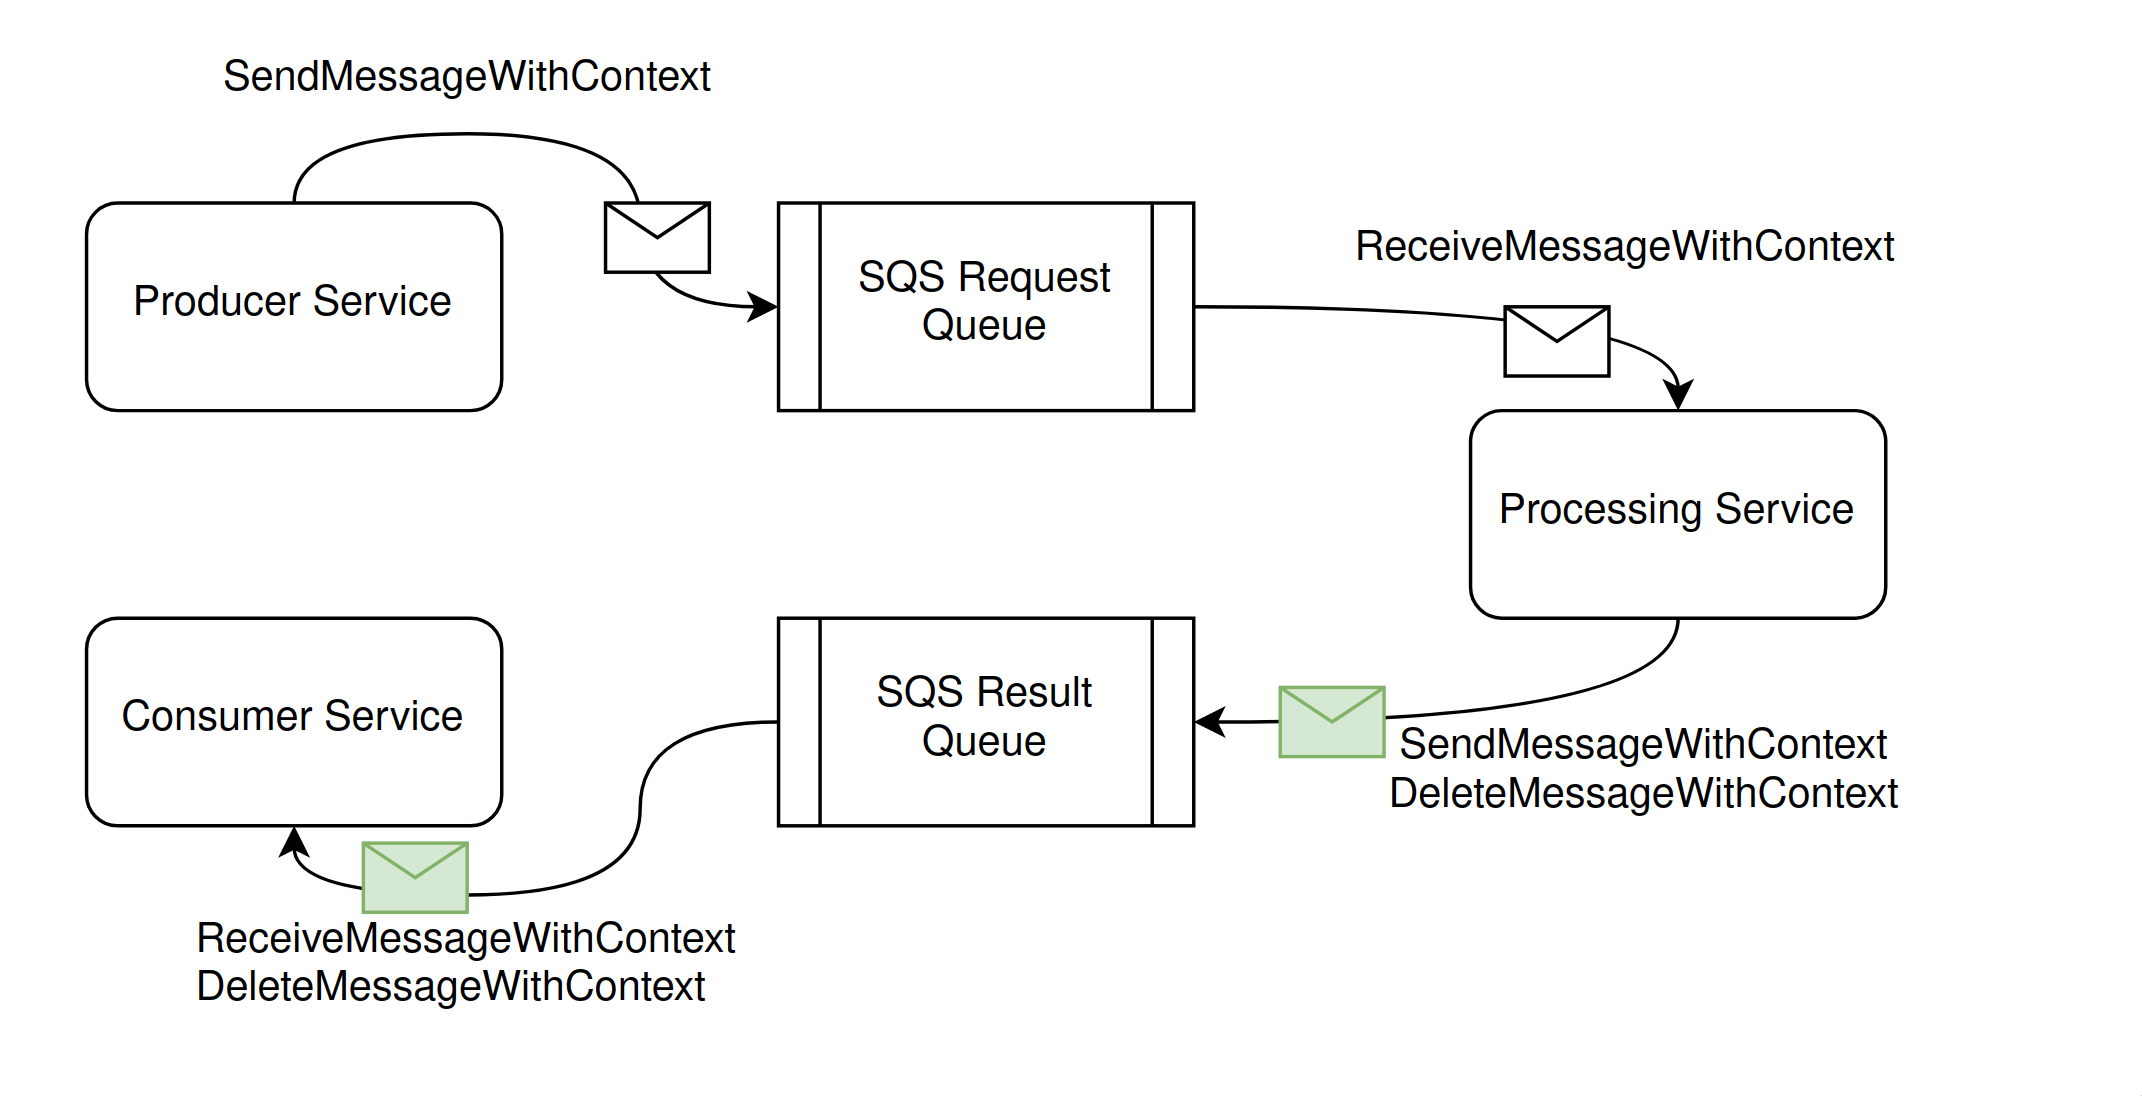
\includegraphics[width=0.95\textwidth]{img/sqs.png}
  \caption{--- SQS}
    \label{fig:sqs}
\end{figure}

\section{Вывод}
Из вышеперечисленного можно сделать вывод, что внедрение микросервисных практик не несет само по себе
каких-то однозначных преимуществ, а скорее является вынужденной мерой при развитии проектов и увеличении их кодовой базы.
В случае, когда:
\begin{enumerate}
    \item предприняты меры по анализу функций приложения для дальнейшего выделения
    логически независимых частей
    \item адаптированы общепринятые практики, связанные с развертыванием и оркестрацией сервисов, упрощающие 
    релизный цикл большого количества компонент
    \item налажены процессы тестирования и документации функциональности сервисов
    \item применяются stateless подходы к разработке сервисов и используются протоколы, обеспечивающие обратную совместимость
    \item уделено время по обеспечению консистентности данных в персистентных хранилищах
    \item используются механизмы кэширования, ретраев и балансировки для повышения надежности и снятия нагрузки сервисов
\end{enumerate}
Можно говорить о потенциальных преимуществах использования микросервисной архитектуры.
Исходя из количества мероприятий, которые требуются для эффективной эксплуатации распределенных систем,
стоит избегать деления на микросервисы в начале развития проекта, но проектировать системы,
имея в виду перспективы дальнейшего редизайна.

В случае перехода на микросервисную архитектуру зрелого приложения не стоит прерывать выстроенные процессы или пытаться
изменить архитектуру в рамках одной итерации. Подход, при котором изменения по разделению логики приложения распределяются
в отдельно развертываемые компоненты происходят инкрементально, называют переходом к удушающему приложению. Так проводится аналогия
с вьюном, который постепенно занимает все жизненное пространство. Аналогично первоначальный монолит распадается на отдельные микросервисы, пока
сам не становится микросервисом.
\section{Основные инструменты построения распределенных архитектур}

Одним из ключевых вопросов при построении распределенных архитектур является асинхронная коммуникация
между миросервисами, которая позволяет независимо масштабировать ее компоненты.

Брокер сообщений является критически важным компонентом при проектировании архитектуры микросервисов. Работая как посредник при передаче данных между различными сервисами, он позволяет минимизировать прямые связи и обеспечивает ряд ключевых преимуществ, которые облегчают разработку, масштабирование и поддержку сложных микросервисных систем.

Одно из основных преимуществ использования брокера сообщений - декуплинг различных компонентов системы. В архитектуре микросервисов декуплинг является важным фактором в обеспечении независимости каждого из сервисов. Благодаря брокеру сообщений, компоненты в системе не должны прямо общаться друг с другом, что повышает их изоляцию и позволяет им работать независимо. Это упрощает процесс обновления или модификации отдельных компонентов, поскольку минимизирует риск сбоев всей системы из-за изменений в одном из сервисов.

Далее, использование брокера сообщений увеличивает надежность системы. Благодаря использованию промежуточного слоя для передачи сообщений, они могут быть надежно сохранены и переданы даже при временных сбоях приема или трансляции. Это гарантирует, что важные данные не будут потеряны из-за сбоев или проблем с конкретными сервисами, усиливая отказоустойчивость всей системы.

Помимо этого, брокеры сообщений обеспечивают асинхронную передачу данных. Это означает, что система не требует немедленного ответа от сервиса-получателя, что может быть критически важно при высоких нагрузках. Брокеры сообщений могут агрегировать сообщения и управлять их доставкой оптимальным образом, обеспечивая более плавную и эффективную работу системы.

На рынке представлено множество различных брокеров сообщений, включая RabbitMQ, Apache Kafka, Google Pub/Sub и AWS Simple Queue Service (SQS). Каждый из этих продуктов предлагает различные функции и возможности, такие как надежные очереди сообщений, модели публикации/подписки, устойчивость к ошибкам и многое другое. Это позволяет разработчикам выбирать наиболее подходящий брокер сообщений для их конкретных нужд и требований.

В итоге, брокеры сообщений играют ключевую роль в архитектуре микросервисов. Они повышают надежность и устойчивость системы, обеспечивают декуплинг между сервисами и позволяют более эффективно управлять данными и нагрузкой в рамках сложных микросервисных экосистем.

Amazon Simple Queue Service (SQS) является мощным инструментом для обработки сообщений в архитектуре микросервисов и обладает несколькими ключевыми преимуществами, которые делают его привлекательным выбором для различных сценариев использования.

Надежность: Amazon SQS предлагает высокую надежность благодаря инфраструктуре Amazon. Сервис гарантирует доставку сообщения хотя бы один раз, что помогает избежать потери данных. Кроме того, Amazon SQS предлагает очереди с повышенной отказоустойчивостью, которые хранят сообщения на протяжении определенного времени, пока они не будут успешно обработаны получателем.

Масштабируемость: Amazon SQS легко масштабируется, чтобы обеспечивать эффективную обработку больших объемов данных. Благодаря возможности бесконечного расширения, этот сервис может гибко настраиваться для поддержки микросервисов любого размера, чтобы поддерживать высокую производительность без дополнительных усилий с вашей стороны.

Безопасность: Благодаря тесной интеграции с AWS Identity and Access Management (IAM), Amazon SQS позволяет точно контролировать доступ к очередям сообщений, обеспечивая высокий уровень безопасности. Также доступны функции транзитного шифрования для дополнительной защиты данных.

Простота использования: Amazon предлагает удобные инструменты для работы с SQS, включая AWS Management Console, SDK и CLI. Это обеспечивает простой метод создания и управления очередями, отправки и приема сообщений и т. д.

Тонкая настройка и контроль: Amazon SQS позволяет настраивать множество параметров очереди, таких как максимальный размер сообщения, период видимости и период удержания, что позволяет оптимизировать сервис под конкретные потребности.

Интеграция с AWS: Если вы уже используете другие сервисы от AWS, такие как Lambda, S3 или EC2, использование SQS значительно упрощает интеграцию микросервисов, поскольку все они работают вместе без каких-либо существенных проблем.

Таким образом, Amazon SQS представляет собой отличный выбор для обработки сообщений в архитектуре микросервисов благодаря своей надежности, масштабируемости, безопасности и простоте использования. Благодаря настройке под конкретные потребности и легкой интеграции с другими сервисами AWS, SQS может стать очень ценным активом в микросервисной архитектуре.
\chapter{РАСПРЕДЕЛЕННАЯ МИКРОСЕРВИСНАЯ АРХИТЕКТУРА ГЕНЕРАЦИИ ИЗОБРАЖЕНИЙ}
\section{Распределенная микросервисная архитектура генерации изображений}
Исходя из перечисленных требований в предыдущей главе архитектура должна:
\begin{enumerate}
    \item Предоставлять возможность горизонтального масштабирования каждой из частей системы по отдельности.
    \item Предоставлять возможность инструментации для диагностики и сбора статистики.
    \item Использовать сетевой транспорт, который обеспечивает отказоустойчивость и оптимальные тайминги сетевых запросов.
    \item Позволять переиспользовать отдельные компоненты другим системам.
\end{enumerate}

В рамках данной работы была реализована система для инференса изображений с HTTP API для внешних потребителей (рис. \ref{fig:design}).

\begin{footnotesize}
\begin{figure}[H]
  \centering
  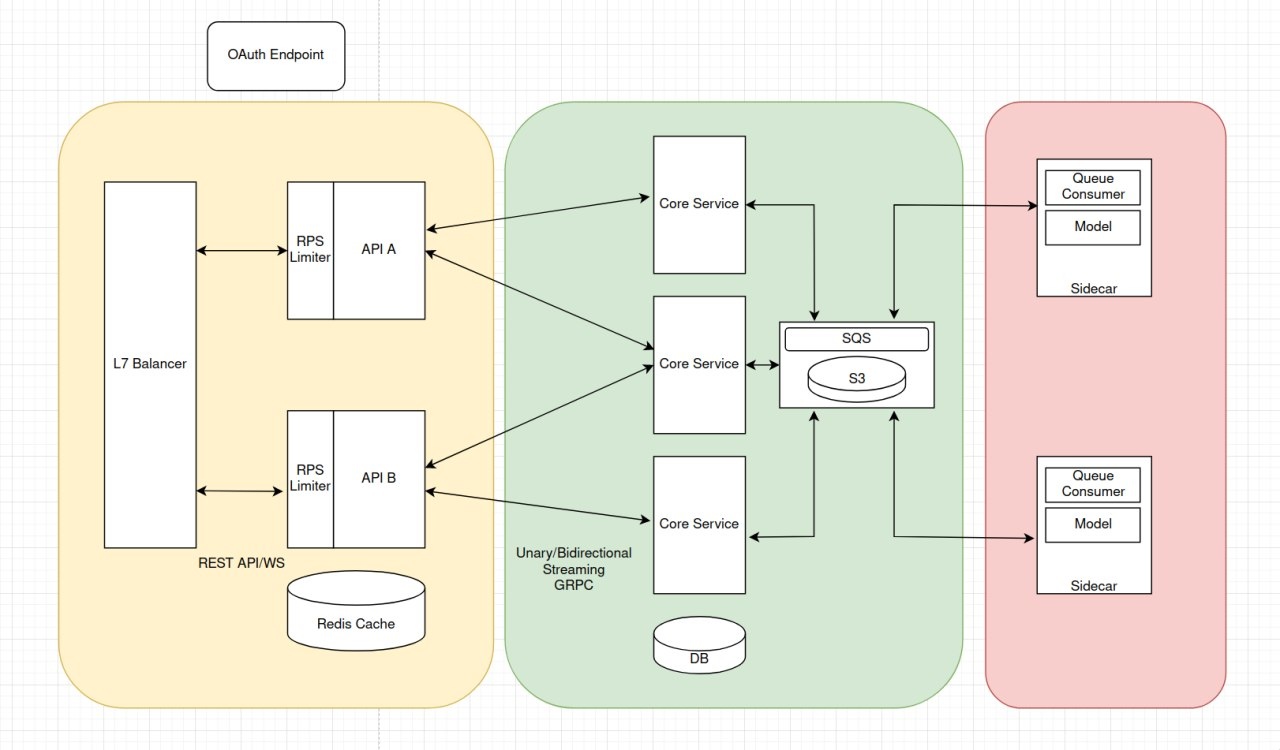
\includegraphics[width=0.95\textwidth]{img/design.png}
  \caption{--- Схема архитектуры}
    \label{fig:design}
\end{figure}
\end{footnotesize}

Данная система состоит из трех основных частей:
\begin{enumerate}
    \item HTTP Gateway для принятия внешних запросов.
    \item Изолированный backend с холодным хранилищем пользовательских запросов генерации.
    \item Сайдкар генерации с моделью генерации изображений с помощью нейронной сети.
\end{enumerate}

HTTP Gateway, представленный желтой зоной на рисунке \ref{fig:design}, предоставляет внешний слой приложения, который отвечает за бизнес-логику,
работу с пользовательскими данными и идентификаторами и проксирует GRPC запросы походами в основной backend.
Как правило, данная часть является наименее нагруженным компонентом системы, поэтому может быть 
представлена единичными экземплярами в каждой из локаций, известных L3 балансеру приложения.

Изоляция данного слоя также позволяет разделять источники траффика в систему и вводить разные
правила на количество поступающих запросов и отдельно кэшировать ответы основного бэкенда.

На данном слое также представляется возможным размещение документации для разработчиков, которые работают
с внешним API системы (рис. \ref{fig:swag}).

\begin{footnotesize}
\begin{figure}[H]
  \centering
  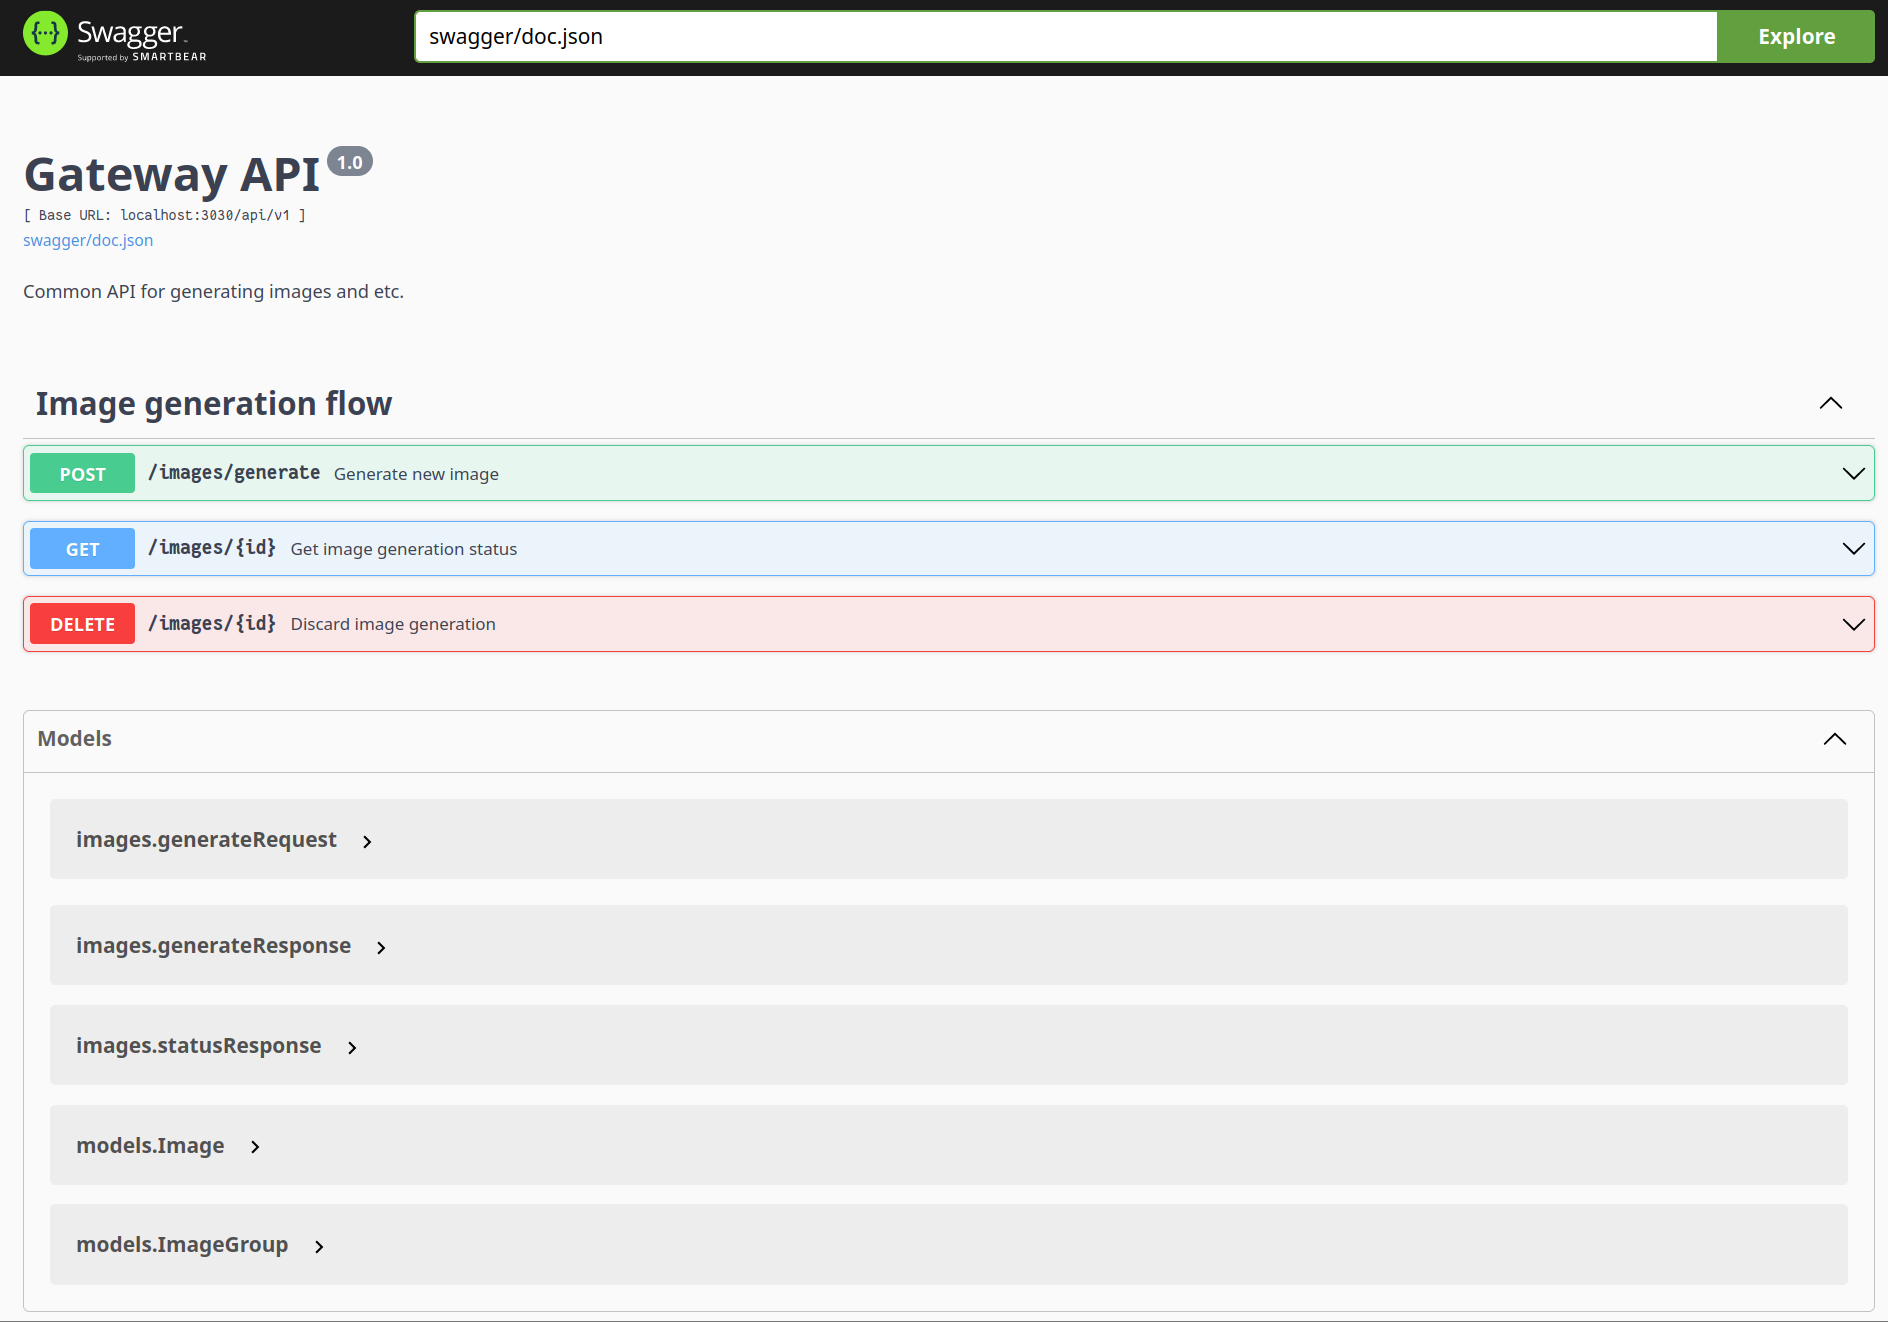
\includegraphics[width=0.95\textwidth]{img/swag.png}
  \caption{--- Внешняя документация эндпоинтов API}
    \label{fig:swag}
\end{figure}
\end{footnotesize}

Итого, HTTP Gateway собирает необходимую информацию из пользовательского запроса и осуществляет сетевой
поход по GRPC в основной backend с нужными параметрами.

Основной backend принимает запросы от HTTP-прокси и осуществляет все сетевые походы во внешние сервисы для
их обслуживания. Для хранения информации об активных запросах, которые обрабатываются асинхронно, необходимо персистентное 
хранилище в виде, например, реляционной базы данных. В данном примере используется YDB, которая является реляционной базой данных.
Также при локальных запусках используется SQlite, поскольку она не требует запуска отдельного контейнера
с исполняемым файлом

Помимо текстовых данных в этом узле системы необходимо работать с бинарными данными, например, изображениями, которые
не рекомендуется хранить в реляционных базах данных. Одним из самых популярных вариантов хранения подобных данных
является AWS S3 (Simple Storage Service). Делегирование хранения бинарных статичных данных в подобный сервис позволяет
использовать CDN для кэширования наиболее востребованных файлов, что предоставляет оптимальное время загрузки данных на клиенте.

Внутренний backend приводит пользовательские HTTP запросы в версионируемые сообщения в Protobuf формате и
записывает в SQS очередь, которую читает сайдкар генерации. Сайдкар генерации занимается непосредственным общением
с моделью нейронной сети, которые зачастую требуют GPU ресурсы, которые менее доступны, чем CPU и RAM, поэтому
количество сайдкаров можно масштабировать назависимо от основного backend-а по количеству доступных GPU.

При реализации взаимодействия между потребителем очереди, который может быть написан на платформе, отличной
от рантайма инференса, возникают различные варианты реализации.

В случае наличия биндингов к рантайму инференса сайдкар может не производить межпроцессного взаимодействия
и коммуницировать с моделью прямо в памяти (рис \ref{fig:side1}). Подобные варианты возможны при использовании 
общеизвестных рантаймов, типа TRT, Onnx и так далее, поскольку биндинги доступны для большого числа платформ.
Однако это требует сохранения модели в установленном формате, что не всегда подходит для произвольной модели.


\begin{footnotesize}
\begin{figure}[H]
  \centering
  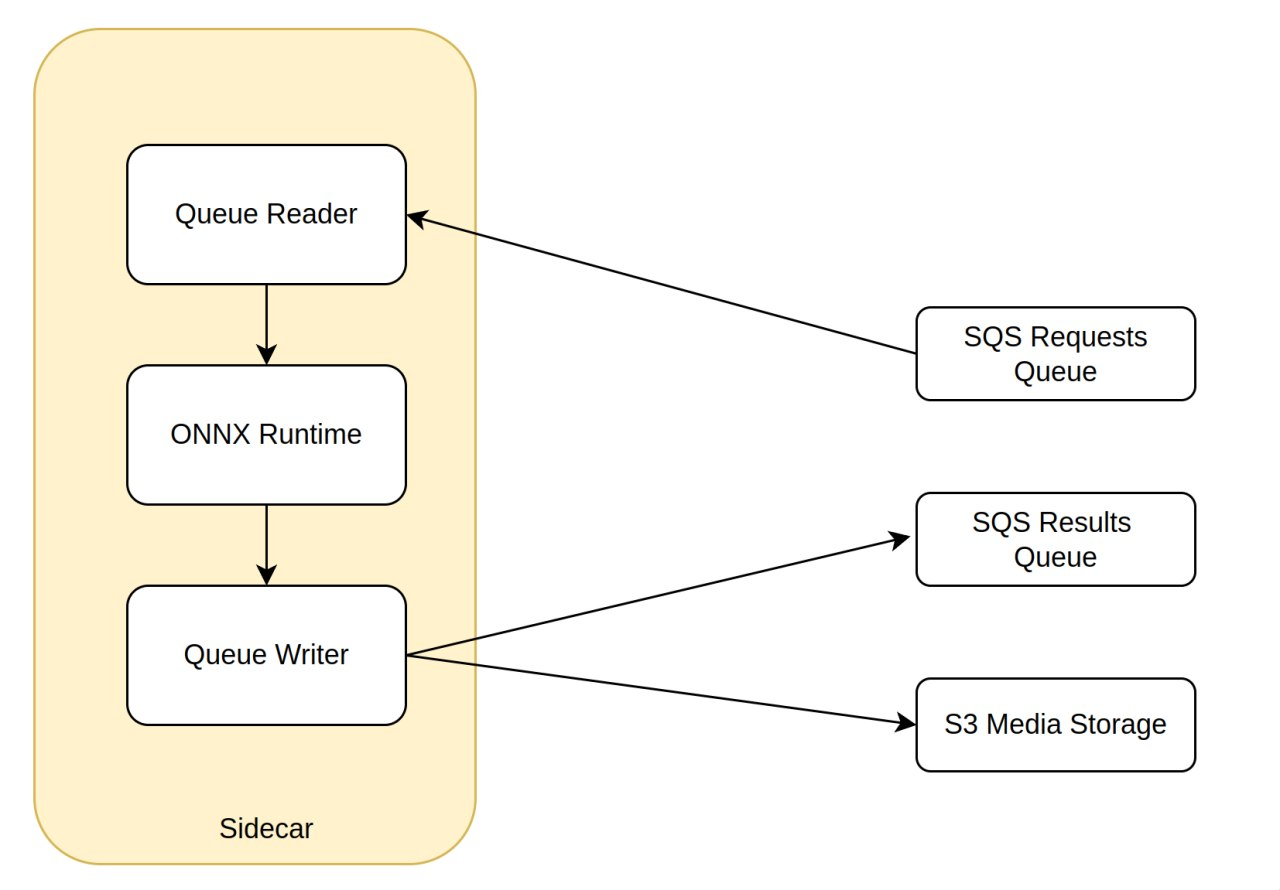
\includegraphics[width=0.95\textwidth]{img/side1.jpg}
  \caption{--- Нативный способ общения с моделью}
    \label{fig:side1}
\end{figure}
\end{footnotesize}

В случаях, когда отсутствует реализация биндигов рантайма модели к основному языку бэкенда,
можно прибегнуть к сетевой передаче данных по HTTP (рис. \ref{fig:side2}). Достоинство данного метода
заключается в простоте использования и внедрения. Данный подход не требует особого формата модели и может
быть использован с верхнеуровневым кодом инференса. В то же время данный подход может не подойти
в ситуациях, где предъявляются строгие требования к latency запросов, потому что передача крупных
бинарных файлов медленнее передачи их по памяти процесса.

\begin{footnotesize}
\begin{figure}[H]
  \centering
  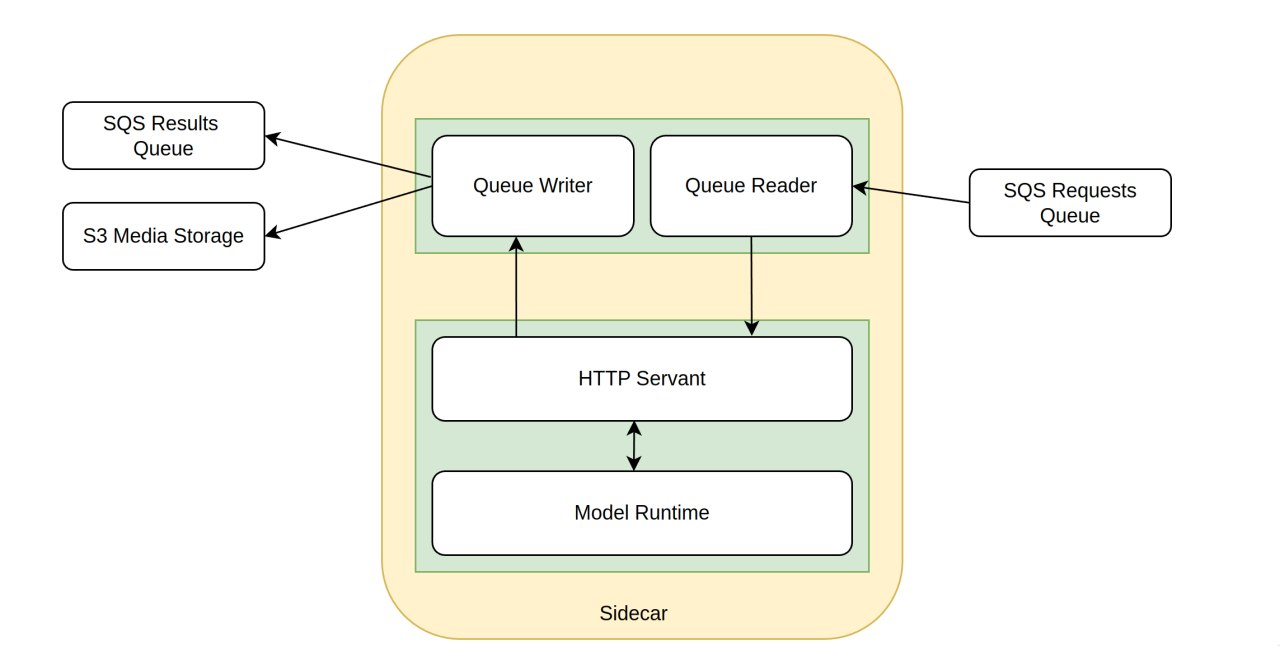
\includegraphics[width=0.95\textwidth]{img/side2.jpg}
  \caption{--- Общение по HTTP с моделью}
    \label{fig:side2}
\end{figure}
\end{footnotesize}

Еще одним способом передачи данных по сети является общение по UDS (рис. \ref{fig:side3}), которое семантически похоже
на общение по TCP c точностью до того, что транспорт данных осуществляется непосредственно через 
память ядра операционной системы. Данный способ показывает многократное улучшение в таймингах ответов
по сравнению с передачей данных по HTTP, однако требует реализации сообственного бинарного протокола, что 
затрудняет разработку.

\begin{footnotesize}
\begin{figure}[H]
  \centering
  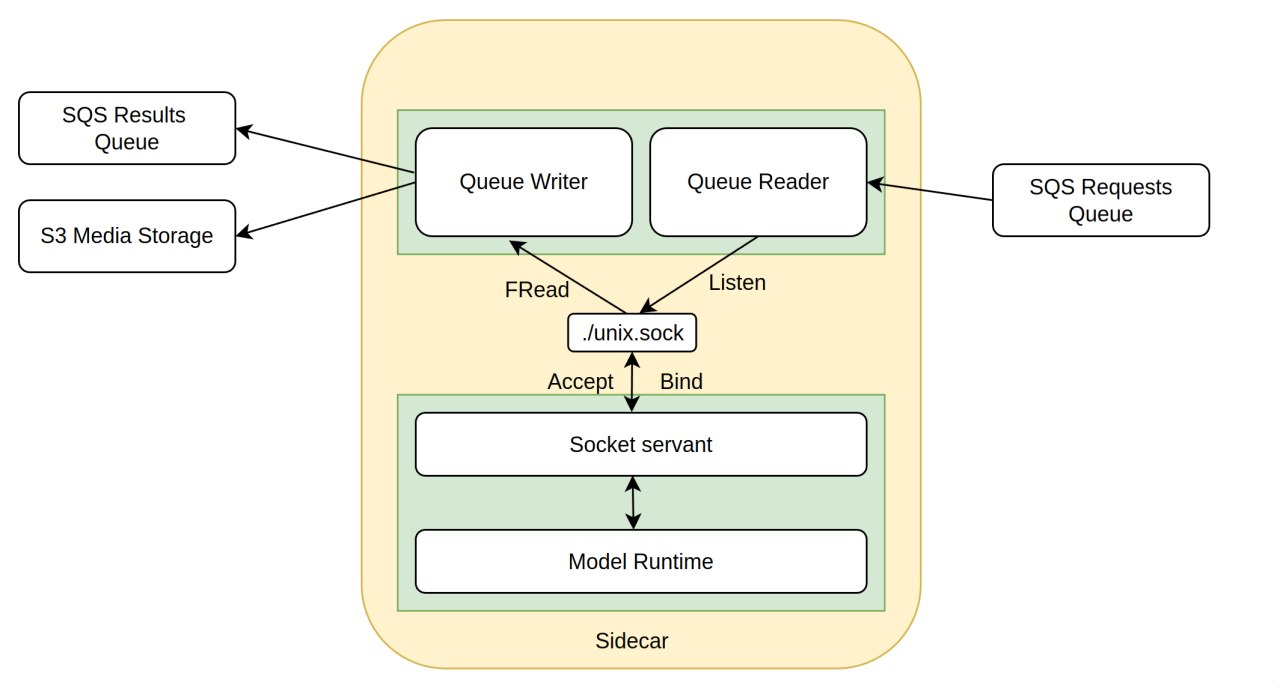
\includegraphics[width=0.95\textwidth]{img/side3.jpg}
  \caption{--- UDS общение с моделью}
    \label{fig:side3}
\end{figure}
\end{footnotesize}

В данном приложении используется взаимодействие через оперативную память, так как
доступен вариант с нативными привязками для Stable Diffusion, которая представляет собой
латентную диффузионную модель.
Инференс Stable Diffusion реализован через C++ библиотеку на основе ggml, что позволяет производить
оптимизированные вычисления на центральном процессоре без видеокарты.
Привязка к собранной библиотеке под C++ для языка Golang осуществляется через поставляемые 
объектные файлы. Данный подход обеспечивает максимальную производительность, но требует 
обработки соглашений вызовов и бинарных API каждой операционной системы. 

В качестве альтернативы применяется также инструмент CGO для языка Golang, который позволяет описывать
символы кода под язык C прямо в коде программ на Golang, что упрощает сборку и разработку, но налагает
значительные ограничения и требует дополнительных ресурсов при переключении контекста между
вызовами процедур на разных языках.

Локальная разработка без выделенных GPU ресурсов обеспечивается за счет уменьшения шагов семплирования
и понижения разрешения изображения, которое необходимо сгенерировать. В случаях, когда не требовалось
использование реальной модели для исследования ее влияния на всю остальную систему, использовался
отдельный интерфейс, который отдавал заготовленные изображения.

\section{Сценарии использования системы генерации изображений}
По умолчанию запрос на генерацию состоит из следующих шагов:
\begin{enumerate}
  \item Клиент отправляет POST запрос с промптом и параметрами изображения.
  \item HTTP Gateway собирает GRPC запрос и вызывает удаленную процедуру внутреннего backend-а.
  \item Внутренний backend создает запись в реляционной базе данных и кладет запрос на генерацию в очередь сайдкара.
  \item Сайдкар достает запрос из очереди и осуществляет инференс модели.
  \item Полученное изображение перекладывается в S3, а ссылка вместе с индентификаторами генерации отправляется в ответную очередь.
  \item При поступлении ответного сообщения изображение перекладывается из временного бакета S3 в публичный, а у генерации в базе данных обновляется статус.
  \item Клиент, получив идентификатор генерации, осуществляет поллинг хендлера статуса до подтверждения завершения, и в конце получает ссылку на полученнное изображение.
\end{enumerate}

Гарантии на обработку сообщения осуществляются за счет Aknowledge семантики чтения сообщений из очереди. 
В SQS это реализовано через выставление visibility timeout, в течение которого сообщение не может быть заново прочитано другим
потребителем. При успешной обработке сообщение удаляется из очереди. При неуспешной обработке сообщение снова становится 
видим для других потребителей и повторно обрабатывается до удаления из очереди.

При возникновении неопределенного поведения или возникновения неконсистентности данных статус может не обновиться.
Для этого предлагается установить TTL на таблицы, связанные с хранением данных о генерации, для 
возможности проставления соответствующего HTTP статуса в API.

В случае, когда время обработки сообщений превышает интервал, с которым в систему
поступают новые запросы, сообщения становятся в очередь, и время обработки сообщения будет 
включать не только время непосредственной обработки, но и время пребывания в очереди.

Для масштабирования поступающей нагрузки необходимо увеличивать количество сайдкаров, которые могут 
обрабатывать очередь независимо друг от друга. Так же уменьшение времени обработки сообщения можно 
достичь за счет батчевания поступающих сообщений: подобная обработка увеличивает время обработки 
каждого отдельного сообщения, но дает выигрыш для группы сообщений, что увеличивает общую
пропускную способность системы.

Как было описано выше, при использовании батчинга можно обрабатывать несколько сообщений одновременно (рис. \ref{fig:flame1})
Однако в этой схеме остаются блокирующие io операции, которые удерживают ресурс GPU во время сборки сообщения и отправки изображений
в S3. 

\begin{footnotesize}

\begin{figure}[H]
  \centering
  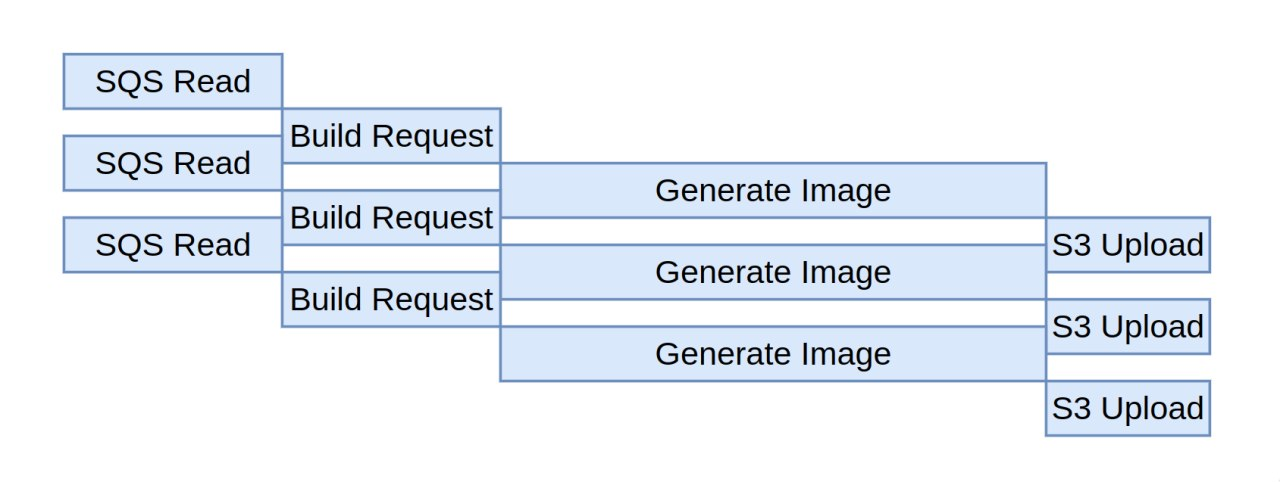
\includegraphics[width=0.95\textwidth]{img/flame1.jpg}
  \caption{--- Батчевая обработка сообщений}
    \label{fig:flame1}
\end{figure}
\end{footnotesize}

Во избежание простоя GPU между отправкой сообщений можно захватывать сообщения наперед
и отправлять их на генерацию во время отправки в S3 (рис. \ref{fig:flame2}).
Данная оптимизация может сэкономить до 200 мс при ожидании в очереди, что составляет
около 5\% от времени генерации изображения в разрешении 256х256 на видеокарте Nvidia Tesla V100.

\begin{footnotesize}
\begin{figure}[H]
  \centering
  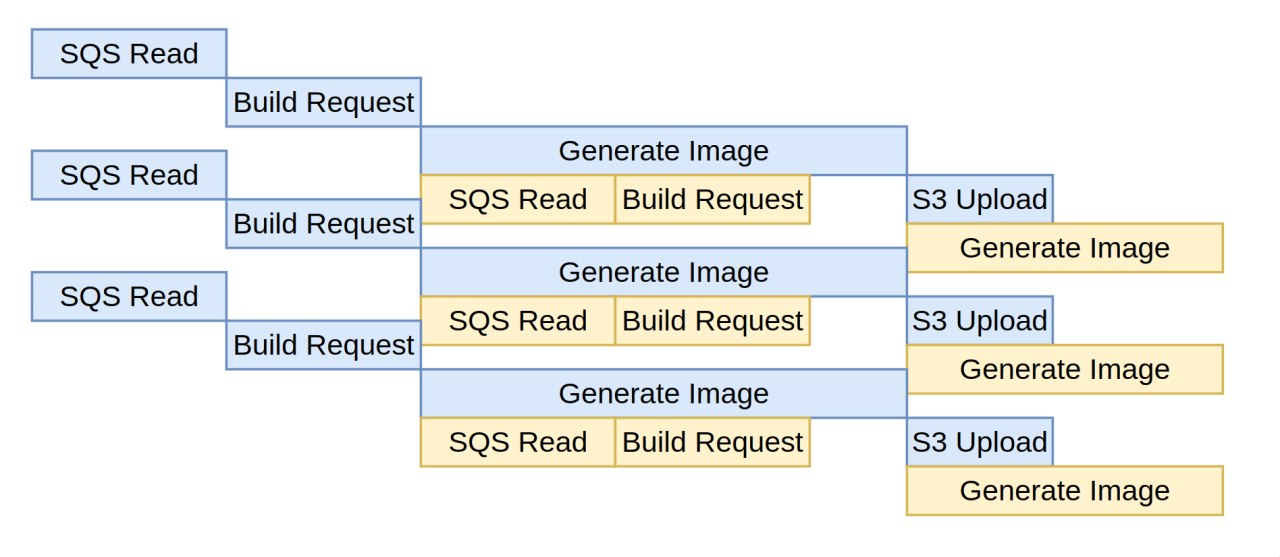
\includegraphics[width=0.95\textwidth]{img/flame2.jpg}
  \caption{--- Батчевая обработка сообщений с захватом очереди}
    \label{fig:flame2}
\end{figure}
\end{footnotesize}
\chapter*{ \large ЗАКЛЮЧЕНИЕ}
\addcontentsline{toc}{chapter}{ЗАКЛЮЧЕНИЕ}

Микросервисная разработка заключается в построении распределенных систем, которые удовлетворяют
критериями масштабируемости и низкой связности отдельных ее узлов.

Она позволяет решать ряд проблем связанных с масштабированием и отказоустойчивостью систем, 
однако налагает ряд ограничений и имеет ряд недостатков, 
которыми приходится сталкиваться в процессе разработки.

Для решения подобных проблем большое внимание уделяется инструментации приложений, описанию контрактов
передачи данных, использованию сетевых и прикладных протоколов, которые обеспечивают гарантии
консистентности данных в зависимости от предъявляемых требований к производительности.

Отдельное внимание также уделяется вопросами инфраструктуры: наличию нескольких зон доступности, 
применению практик непрерывной интеграции, тестирования и использования баз данных и брокеров сообщений,
которые можно горизонтально масштабировать вместе с приложением.

При выполнению предписываемых рекомендаций по внедрению микросервисных архитектур получается
добиться горизонтального масштабирования приложений, распределения сложности системы 
между ее независимыми узлами и выдерживать периоды повышенной нагрузки.

В ходе работы было рассмотрено понятие микросервисной архитектуры и произведен обзор имеющихся средств и подходов разработки,
применяющихся для коммуникации веб-сервисов.

В данной работе также было показано, что микросервисная разработка хорошо подходит для обработки запросов
по генерации изображений, позволяет независимо масштабировать разные виды вычислительных ресурсов и 
позволяет более надежно обрабатывать большое количество запросов при ограниченных ресурсах GPU.

Результатом работы стала разработка программного обеспечения для генерации изображений
с помощью нейронной сети с сетевым интерфейсом, которое представляет собой систему из трех микросервисов,
демонстрирующих различные виды синхронного и асинхронного сетевого взаимодействия, а также технологий,
которые применяются при микросервисной разработке. 

На примере данной системы также рассмотрены проблемы, которые могут возникнуть при технических неполадках
и предложены варианты их решения.


\bibliography{src}
\bibliographystyle{unsrt}

\addcontentsline{toc}{chapter}{СПИСОК ИСПОЛЬЗОВАННОЙ ЛИТЕРАТУРЫ}

\titleformat{\section}[block]
  {\large\bfseries\centering}
  {\thesection\ }{}{}

\titleformat{\chapter}[display]{\normalfont\bfseries\raggedleft}{\chaptertitlename\ \thechapter}{18pt}{\Large}

\chapter*{ПРИЛОЖЕНИЕ А}
\addcontentsline{toc}{chapter}{ПРИЛОЖЕНИЕ А}
\section*{Репозиторий приложения на GitHub}

Код приложения находится в открытом доступе на платформе коллаборации GitHub по ссылке, представленной в виде QR-кода.
Практическая часть, упоминаемая в основной работе, представлена пакетами cmd и internal. Также присутствует docker-compose файлы необходимые для поднятия
нужного окружения с томами для брокера сообщений, базы данных, хранилища медиа-файлов и инструментации приложения.

\begin{footnotesize}
\begin{figure}[h]
  \centering
  
\includegraphics[width=0.69\textwidth]{img/frame.png}
  \caption*{}
\end{figure}

\end{footnotesize}

Далее будут приведены ключевые файлы конфигурации и описания приложения.

\subsection*{Docker compose спецификация для локального запуска микросервисов}
\begin{lstlisting}[]
version: "3.8"

services:
  localstack:
    container_name: "${LOCALSTACK_DOCKER_NAME:-localstack-main}"
    image: localstack/localstack
    ports:
      - "127.0.0.1:4566:4566"
      - "127.0.0.1:4510-4559:4510-4559"
    environment:
      - DEBUG=${DEBUG:-0}
    volumes:
      - "${LOCALSTACK_VOLUME_DIR:-./volume}:/var/lib/localstack"
      - "/var/run/docker.sock:/var/run/docker.sock"

  prometheus:
    image: prom/prometheus:v2.25.0
    volumes:
      - ./prometheus:/etc/prometheus
      - prom_data:/prometheus
    command:
      - '--config.file=/etc/prometheus/prometheus.yml'
    ports:
      - 9090:9090

  grafana:
    image: grafana/grafana:7.5.7
    ports:
      - 3000:3000
    restart: unless-stopped
    volumes:
      - grafana-data:/var/lib/grafana
      - ./grafana:/etc/grafana/provisioning/datasources

  jaeger:
    image: jaegertracing/all-in-one:latest
    environment:
      - COLLECTOR_OTLP_ENABLED=true
    ports:
      - 16686:16686
      - 4318:4318
      - 5778:5778

volumes:
  grafana-data:
  prom_data:
\end{lstlisting}


\subsection*{GRPC спецификация сервиса генерации}
\begin{lstlisting}[]
  syntax = "proto3";

package proto.echo;

option go_package = "./proto";

service Core {
  rpc Generate(GenerateRequest) returns (GenerateResponse);
  rpc Discard(DiscardRequest) returns (DiscardResponse);
  rpc Status(StatusRequest) returns (StatusResponse);
}

message GenerateRequest {
  string Prompt = 1;
}

message GenerateResponse {
  string ID = 2;
}

message StatusRequest {
  string ID = 1;
}

message StatusResponse {
  ImageGroup ImageGroup = 1;
}

message DiscardRequest {
  string ID = 1;
}

message DiscardResponse {
}

message Image {
  string ID = 1;
  string Prompt = 2;
  string URL = 3;
  string Status = 4;
}

message ImageGroup {
  string ID = 1;
  repeated Image Images = 2;
}
\end{lstlisting}


\end{document}

\grid